\documentclass[handout,compress]{beamer}

\usetheme[block=fill]{metropolis}

\usepackage{graphicx} % Allows including images
\usepackage{amsmath,amsfonts,amsthm,amssymb}
\usepackage{color}
\usepackage{xcolor,cancel}
%\setitemize{label=\usebeamerfont*{itemize item}%
%	\usebeamercolor[fg]{itemize item}
%	\usebeamertemplate{itemize item}}
\definecolor{mDarkBrown}{HTML}{604c38}
\definecolor{mDarkTeal}{HTML}{23373b}
\definecolor{mLightBrown}{HTML}{EB811B}
\definecolor{mMediumBrown}{HTML}{C87A2F}
\definecolor{mygreen}{HTML}{98C2B9}
\definecolor{myyellow}{HTML}{DFD79C}
\definecolor{myblue}{HTML}{8CA7CC}
\definecolor{kern}{HTML}{8CC2B7}

\usepackage{float}
\usepackage{framed}
\usepackage{epsfig}
\usepackage{graphicx}
\usepackage{subcaption}
\usepackage{ulem}
\usepackage{hhline}
\usepackage{multirow}
\usepackage{comment}   
\usepackage{bbm}
\usepackage{tikz}   
\usepackage{ulem}
\def\Put(#1,#2)#3{\leavevmode\makebox(0,0){\put(#1,#2){#3}}}
\newcommand*\mystrut[1]{\vrule width0pt height0pt depth#1\relax}
\newcommand{\eqdef}{\mathbin{\stackrel{\rm def}{=}}}


\newcommand{\bs}[1]{\boldsymbol{#1}}
\newcommand{\bv}[1]{\mathbf{#1}}
\newcommand{\R}{\mathbb{R}}
\newcommand{\E}{\mathbb{E}}

\DeclareMathOperator*{\argmin}{arg\,min}
\DeclareMathOperator*{\argmax}{arg\,max}
\DeclareMathOperator{\nnz}{nnz}
\DeclareMathOperator{\Var}{Var}
\DeclareMathOperator{\sinc}{sinc}
\DeclareMathOperator{\mv}{mv}
\DeclareMathOperator{\sgn}{sgn}
\DeclareMathOperator{\step}{step}
\DeclareMathOperator{\gap}{gap}
\DeclareMathOperator{\poly}{poly}
\DeclareMathOperator{\tr}{tr}
\DeclareMathOperator{\orth}{orth}
\newcommand{\norm}[1]{\|#1\|}
\captionsetup[subfigure]{labelformat=empty}
\captionsetup[figure]{labelformat=empty}
\DeclareMathOperator*{\lmin}{\lambda_{min}}
\DeclareMathOperator*{\lmax}{\lambda_{max}}

\newcommand{\specialcell}[2][c]{%
	\begin{tabular}[#1]{@{}c@{}}#2\end{tabular}}
\newcommand{\specialcellleft}[2][c]{%
	\begin{tabular}[#1]{@{}l@{}}#2\end{tabular}
}

\usepackage{tabstackengine}
\stackMath

\newtheorem{claim}[theorem]{Claim}


%----------------------------------------------------------------------------------------
%	TITLE PAGE
%----------------------------------------------------------------------------------------

\title{CS-UY 4563: Lecture 17 \\ Neural Networks cont.}
\author{NYU Tandon School of Engineering, Prof. Christopher Musco}
\date{}

\begin{document}
	
	\begin{frame}
		\titlepage 
	\end{frame}
	
	\metroset{titleformat=smallcaps}
	
	\begin{frame}
		\frametitle{course logistics}
		\begin{itemize}
			\item Lab \texttt{lab\_mnist\_partial.ipynb} due {Thursday, 4/9.}
			\item Project Proposal due next Monday, 4/13. 
			\begin{itemize}
				\item See guidelines for what to include at: \url{https://www.chrismusco.com/introml/project_guidelines.pdf}
				\item Can be crudely formatted. A shared Google doc is fine, or email me a PDF.
				\item I'm seeing lots of really cool project ideas!
			\end{itemize} 
		\end{itemize}
	\end{frame}
	
	\begin{frame}
		\frametitle{training neural networks}
		\textbf{Two main algorithmic tools for training neural network models:}
		\begin{enumerate}
			\item Stochastic gradient descent.
			\item \alert{\textbf{Back-propogation}}.
		\end{enumerate}
	\end{frame}
	
	\begin{frame}
		\frametitle{training neural networks}
		Let $f(\vec{\theta},\vec{x})$ be our neural network. 
		
		$\bv{W}_{i}$ and $\vec{b}_i$ are the \emph{weight matrix} and \emph{bias vector} for layer $i$ and $g_i$ is the non-linearity (e.g. sigmoid). $\vec{\theta} = [\bv{W}_0,\vec{b}_0, \ldots,\bv{W}_\ell,\vec{b}_\ell]$ is a vector of all entries in these matrices.
		
		\textbf{Goal:} Given training data $(\vec{x}_1, y_1),\ldots,(\vec{x}_n, y_n)$ minimize the loss
		\begin{align*}
		\mathcal{L}(\vec{\theta}) = \sum_{i=1}^n L\left(y_i,f(\vec{\theta}, \vec{x}_i)\right)
		\end{align*}
		
		\begin{center}
			\alert{\textbf{To do so, we need to compute $\nabla L\left(y_i,f(\vec{\theta}, \vec{x}_i)\right)$ for all $i$.}}
		\end{center} 
	\end{frame}
	
	\begin{frame}
		\frametitle{gradient of the loss}
		\textbf{Last lecture:} Reduced our goal to computing $\nabla f(\vec{\theta}, \vec{x})$, where the gradient is with respect to the parameters $\vec{\theta}$.
		
		This will be done using backprop.
	\end{frame}
	
	\begin{frame}
		\frametitle{backprop example}
		\small
		\vspace{-.5em}
		\begin{center}
			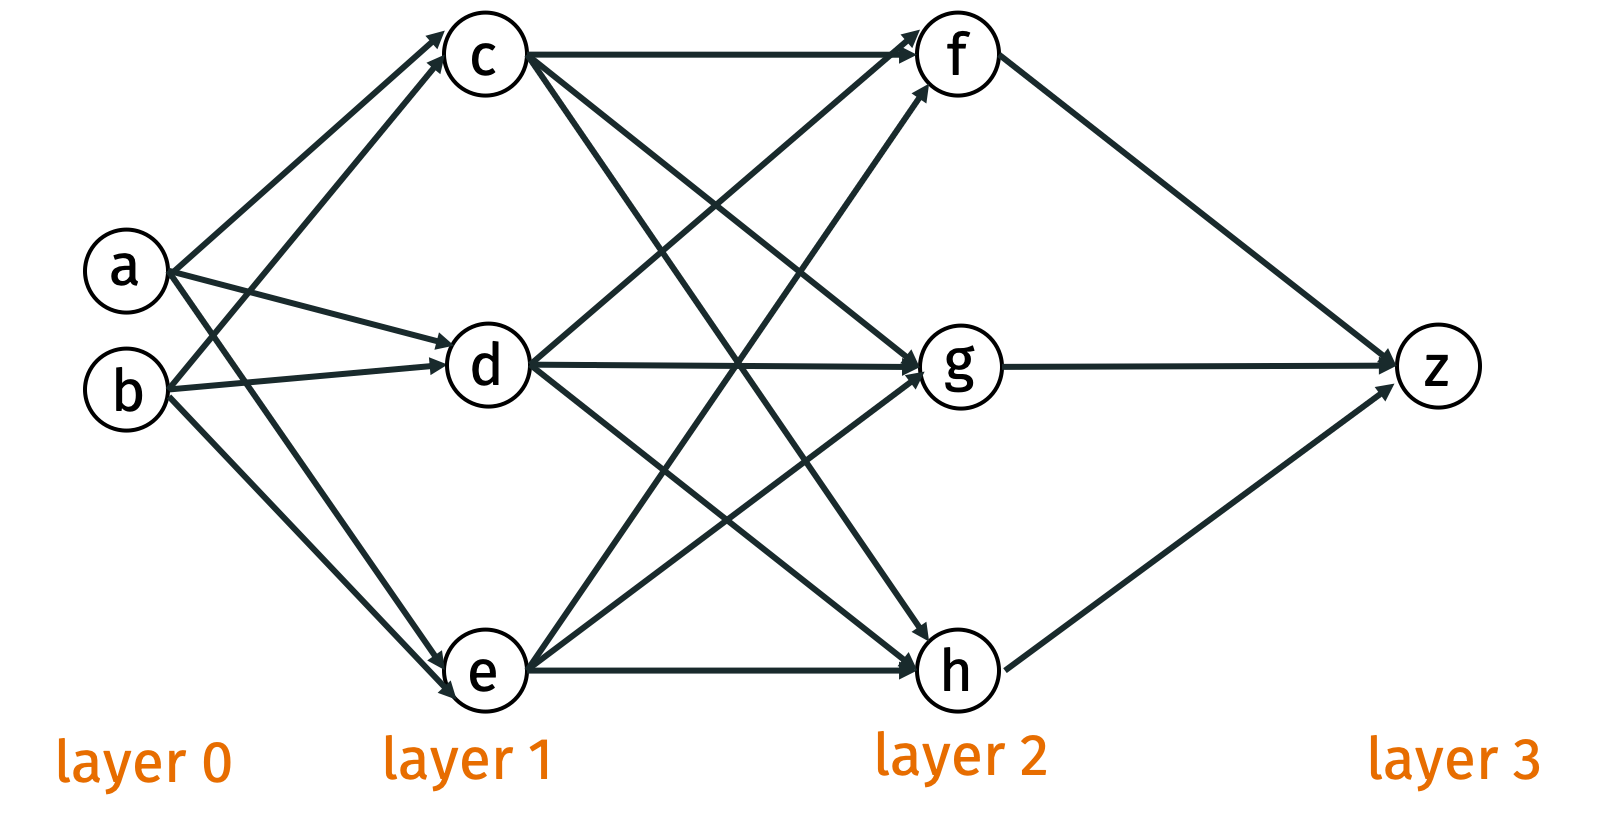
\includegraphics[width=.6\textwidth]{backpro_example.png}
			\vspace{-1em}
		\end{center}
		Notation for next few slides:
		\vspace{-1em}
		\begin{itemize}
			\item $a, b, \ldots, z$ are the node names, and used to denote values at nodes after applying non-linearity.
			\item $\bar{a}, \bar{b}, \ldots, \bar{z}$ denote value before applying non-linearity.
			\item $W_{i,j}$ is the weight of edge from node $i$ to node $j$. 
			\item $s(\cdot): \R\rightarrow \R$ is the non-linear activation function. 
			\item $\beta_{j}$ is the bias for node $j$.
		\end{itemize}
		\textbf{Example:} $h = s(\bar{h}) = s(c\cdot W_{c,h} + d\cdot W_{d,h} + e\cdot W_{e,h} + \beta_h)$
	\end{frame}
	
	\begin{frame}
		\frametitle{backprop example}
		\textbf{Goal:} Compute the gradient $\nabla f(\vec{\theta},\vec{x})$, which contains the partial derivatives with respect to \emph{every} parameter:
		\begin{itemize}
			\item $\partial z / \partial \beta_z$
			\item $\partial z / \partial W_{f,z}$, $\partial z / \partial W_{g,z}$, $\partial z / \partial W_{h,z}$
			%		\item $\partial z / \partial \beta_f$, $\partial z / \partial  \beta_g$, $\partial z / \partial \beta_h$
			\item $\partial z / \partial W_{c,f}$, $\partial z / \partial W_{c,g}$, $\partial z / \partial W_{c,h}$
			\item $\partial z / \partial W_{d,f}$, $\partial z / \partial W_{d,g}$, $\partial z / \partial W_{d,h}$
			\item $\vdots$
			\item $\partial z / \partial W_{a,c}$, $\partial z / \partial W_{a,d}$, $\partial z / \partial W_{a,e}$
		\end{itemize}
		\textbf{Two steps:} \emph{Forward pass} to compute function value. \emph{Backwards pass} to compute gradients. 
	\end{frame}
	
	\begin{frame}
		\frametitle{backprop example}
		\textbf{Step 1:} Forward pass. 
		\begin{center}
			\vspace{-.5em}
			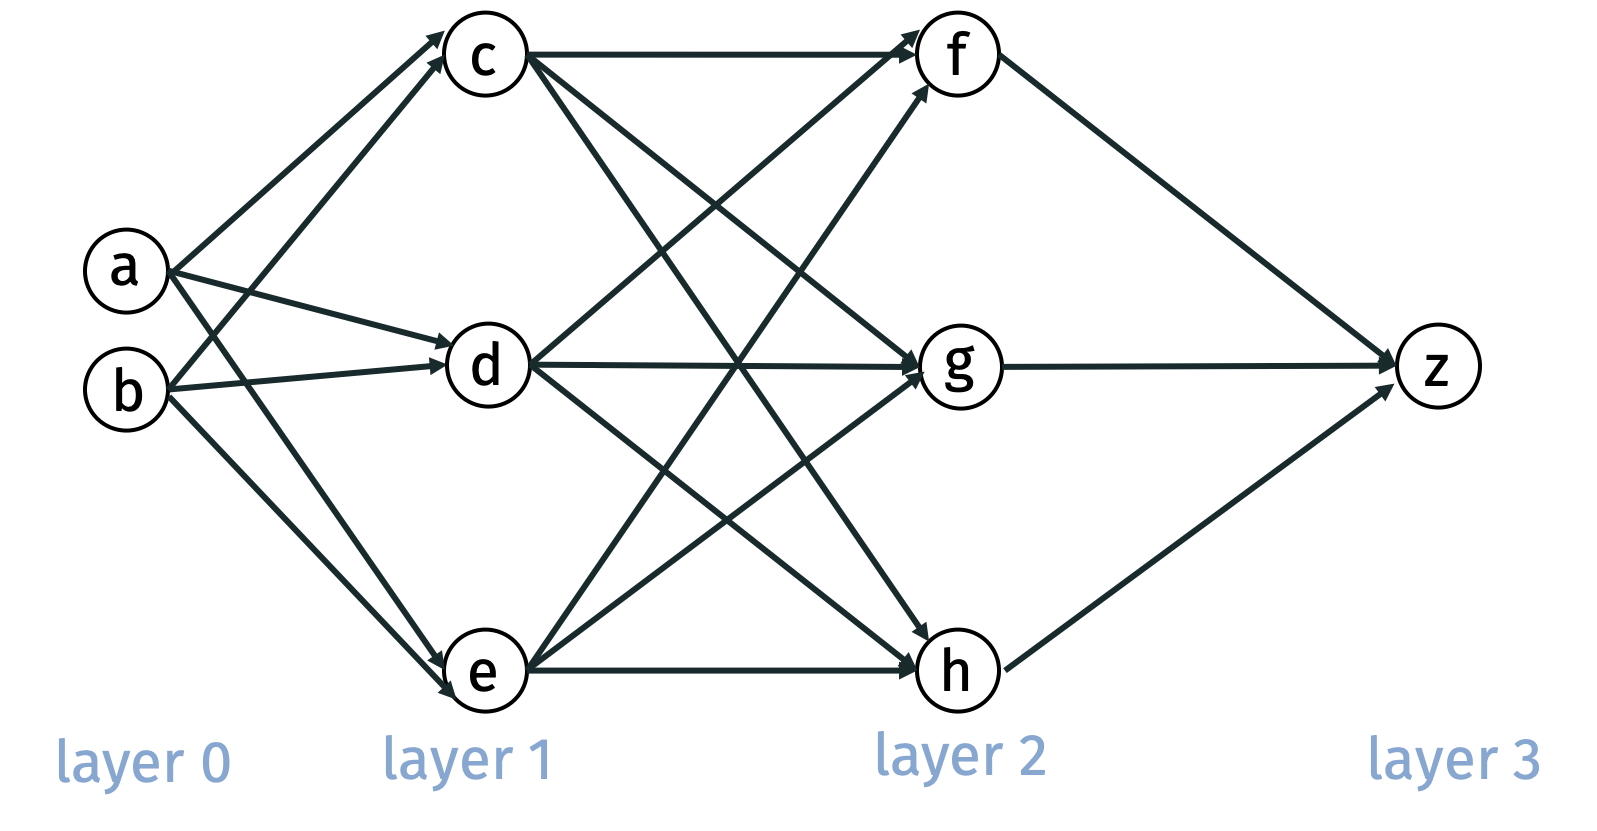
\includegraphics[width=.6\textwidth]{no_select.png}
			\vspace{-1em}
		\end{center}
		\begin{itemize}
			\item Using \textbf{current parameters}, compute the output $z$ by moving from left to right.
			\item Store all intermediate results: \begin{align*}\bar{c}, \bar{d}, \bar{e}, c,d,e, \bar{f}, \bar{g}, \bar{h}, f,g,h, \bar{z}, z. \end{align*}
		\end{itemize}	
	\end{frame}
	
	\begin{frame}[t]
		\frametitle{backprop example}
		\small
		\textbf{Step 1:} Forward pass. 
		
		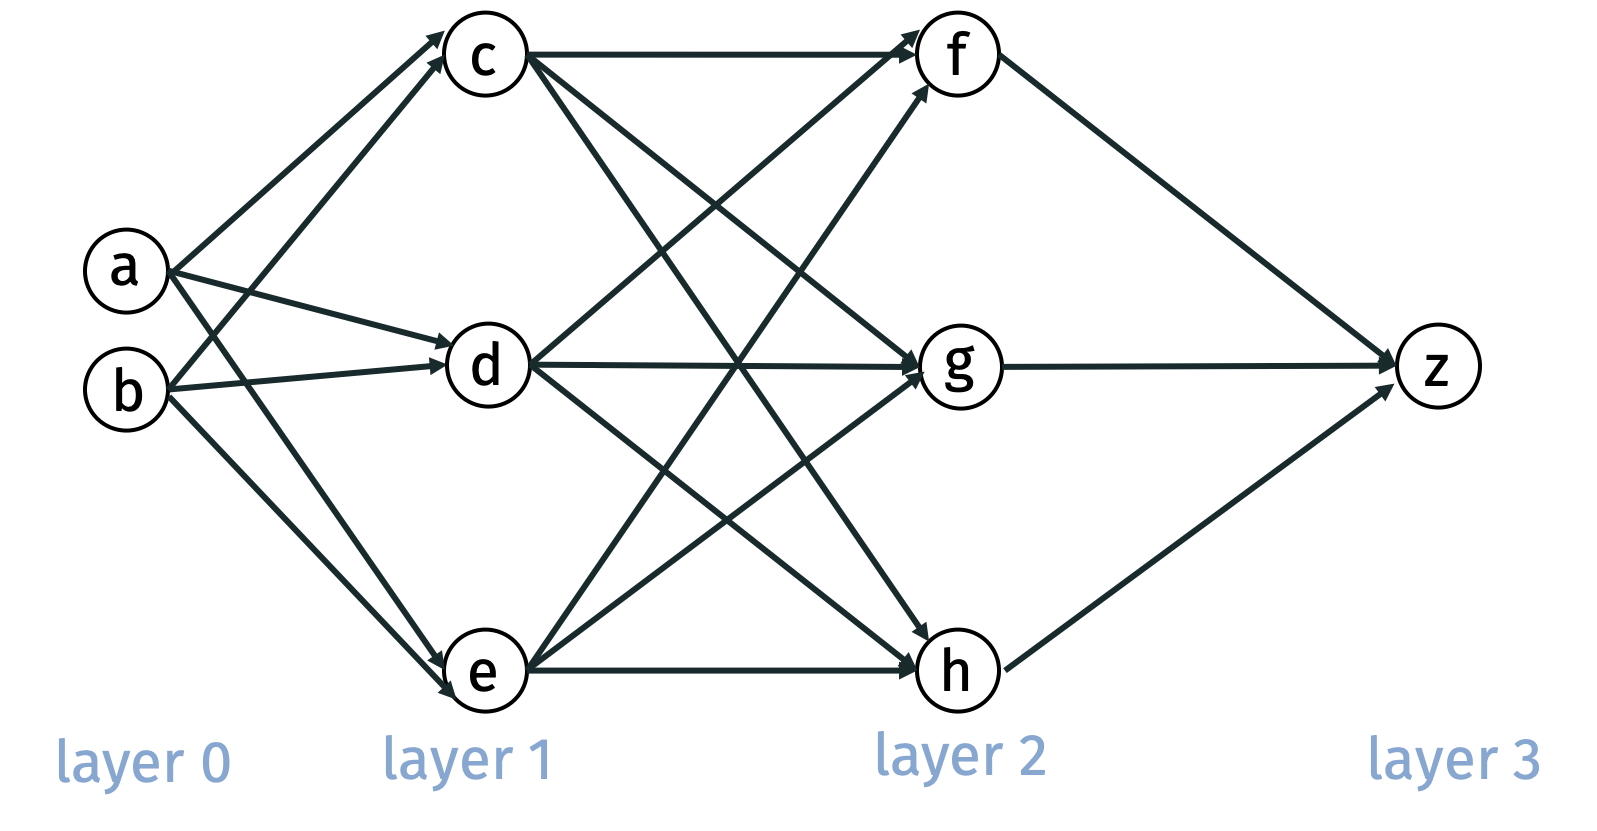
\includegraphics[width=.5\textwidth]{no_select.png}
		\begin{align*}
		\bar{c} &= W_{a,c}\cdot a + W_{b,c}\cdot b + \beta_c & c&= s(\bar{c})\\
		\bar{d} &= W_{a,d}\cdot a + W_{b,d}\cdot b + \beta_d & d&= s(\bar{d})\\
		\bar{e} &= W_{a,e}\cdot a + W_{b,e}\cdot b + \beta_e & e&= s(\bar{e})\\
		\bar{f} &= W_{c,f}\cdot c + W_{d,f}\cdot d + W_{e,f}\cdot e + \beta_f & f&= s(\bar{f})
		\\
		&\vdots & &\vdots\\
		\bar{z} &= W_{f,z}\cdot f + W_{g,z}\cdot g + W_{h,z}\cdot h + \beta_z & z&= s(\bar{z})
		\end{align*}
	\end{frame}
	
	\begin{frame}
		\frametitle{backprop example}
		\textbf{Step 2:} Backward pass. 
		\begin{center}
			\vspace{-.5em}
			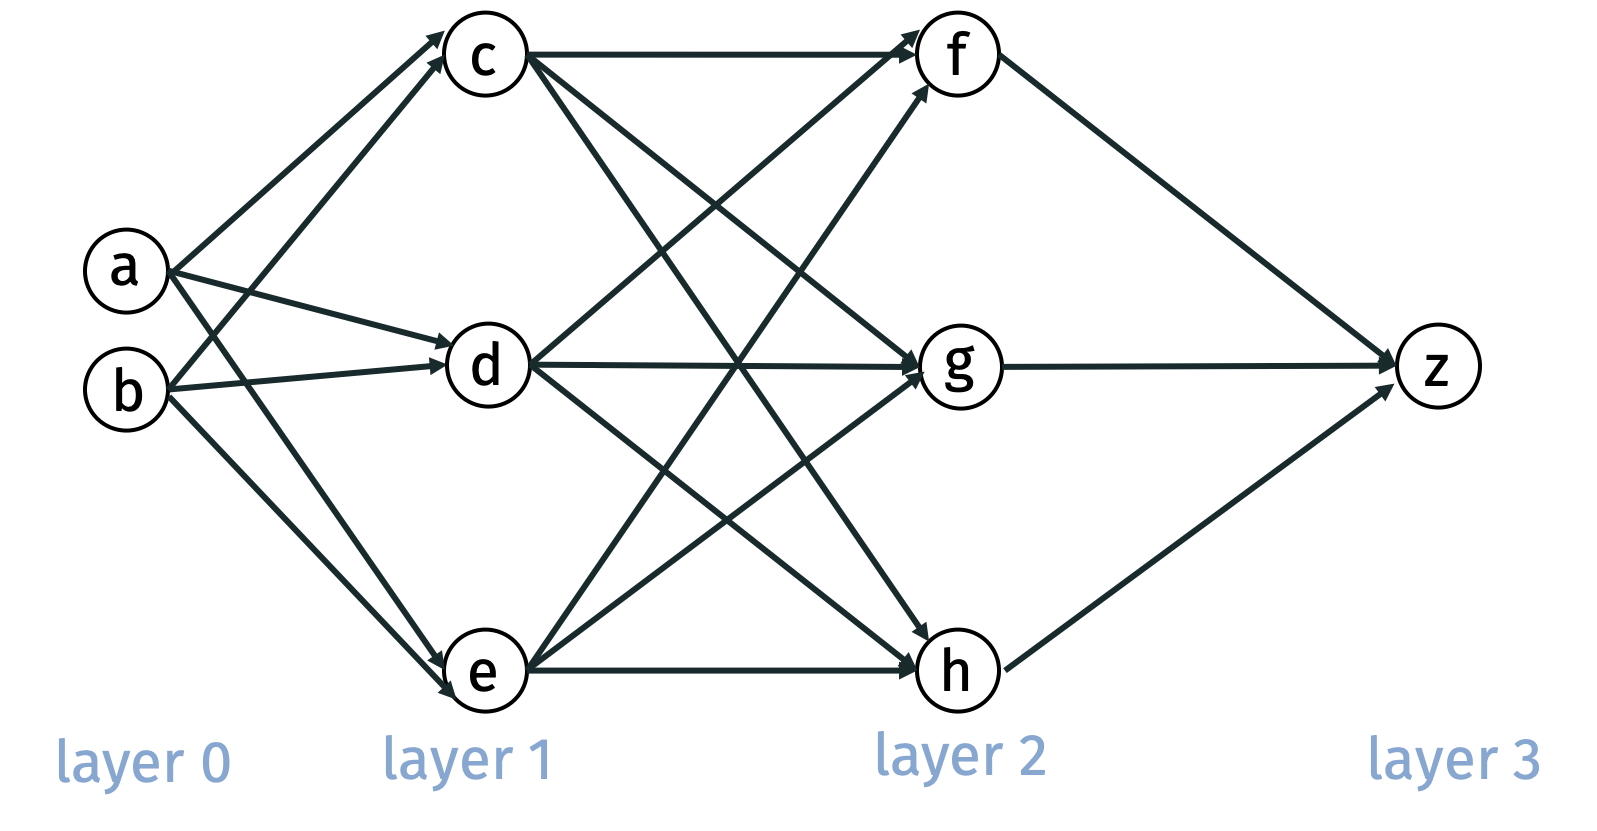
\includegraphics[width=.6\textwidth]{no_select.png}
			\vspace{-1em}
		\end{center}
		\begin{itemize}
			\item Using \textbf{current parameters} and \textbf{computed node values}, compute the partial derivatives of all parameters by moving from \emph{right to left}.
		\end{itemize}	
	\end{frame}
	
	\begin{frame}[t]
		\frametitle{backprop example}
		\small
		\textbf{Step 2:} Backward pass. Deepest layer.
		
		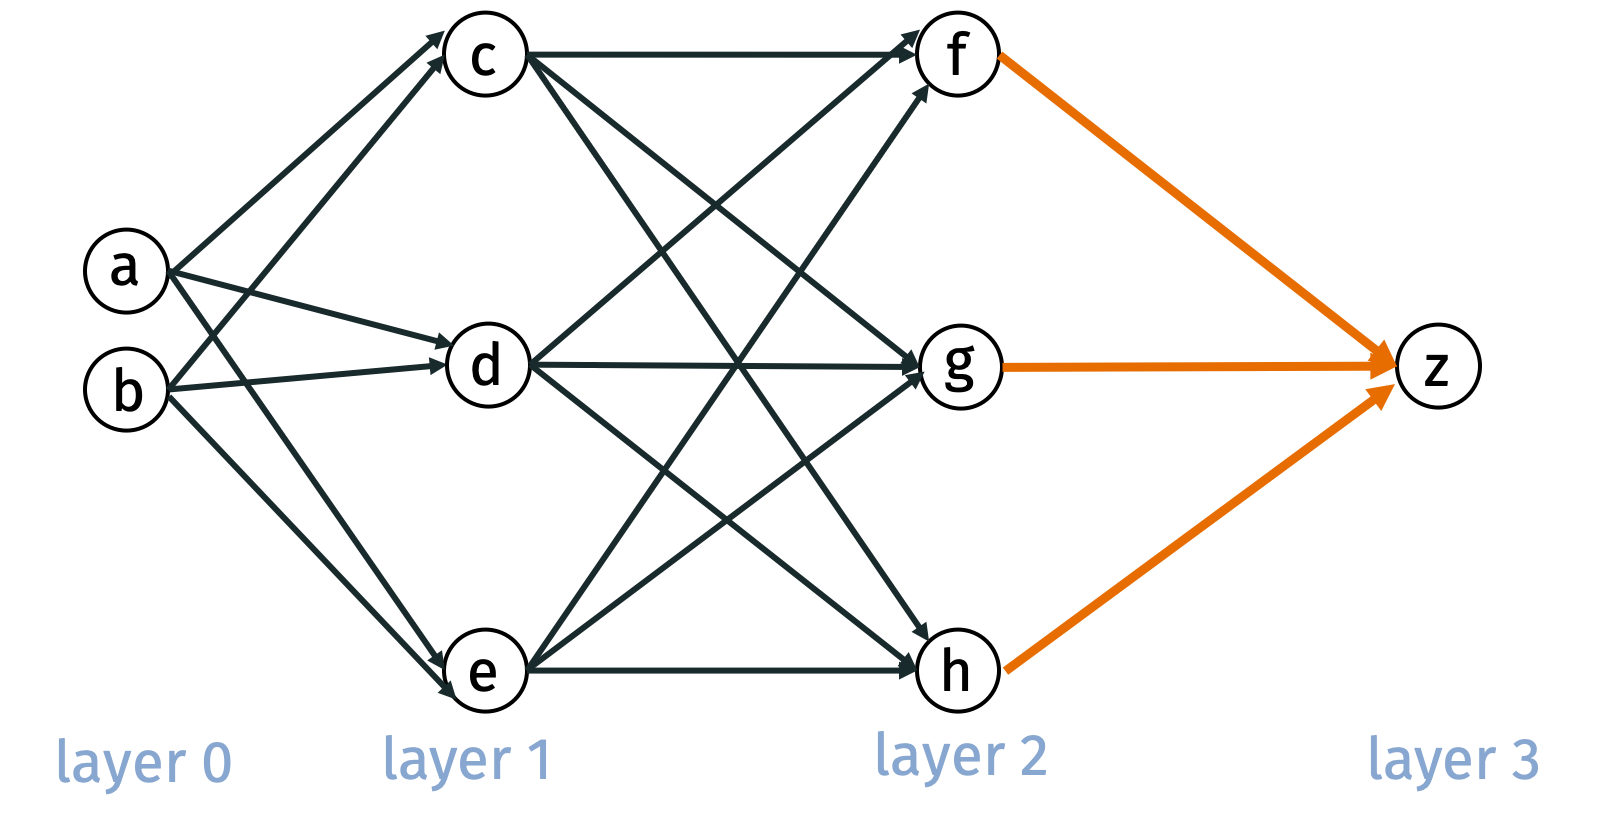
\includegraphics[width=.5\textwidth]{layer1.png}
		\begin{align*}
		\alert{\frac{\partial z}{\partial b_{z}}} &= \frac{\partial \bar{z}}{\partial b_{z}}\cdot \frac{\partial z}{\partial \bar{z}} = 1\cdot s'(\bar{z})\\
		\alert{\frac{\partial z}{\partial W_{f,z}}} &= \frac{\partial \bar{z}}{\partial W_{f,z}}\cdot \frac{\partial z}{\partial \bar{z}} = f\cdot s'(\bar{z}) \\
		\alert{\frac{\partial z}{\partial W_{g,z}}} &= \frac{\partial \bar{z}}{\partial W_{g,z}}\cdot \frac{\partial z}{\partial \bar{z}} = g\cdot s'(\bar{z}) \\
		\alert{\frac{\partial z}{\partial W_{h,z}}} &= \frac{\partial \bar{z}}{\partial W_{h,z}}\cdot \frac{\partial z}{\partial \bar{z}} = h\cdot s'(\bar{z})
		\end{align*}
	\end{frame}

	\begin{frame}[t]
	\frametitle{backprop example}
	\small
	\textbf{Step 2:} Backward pass.
	
	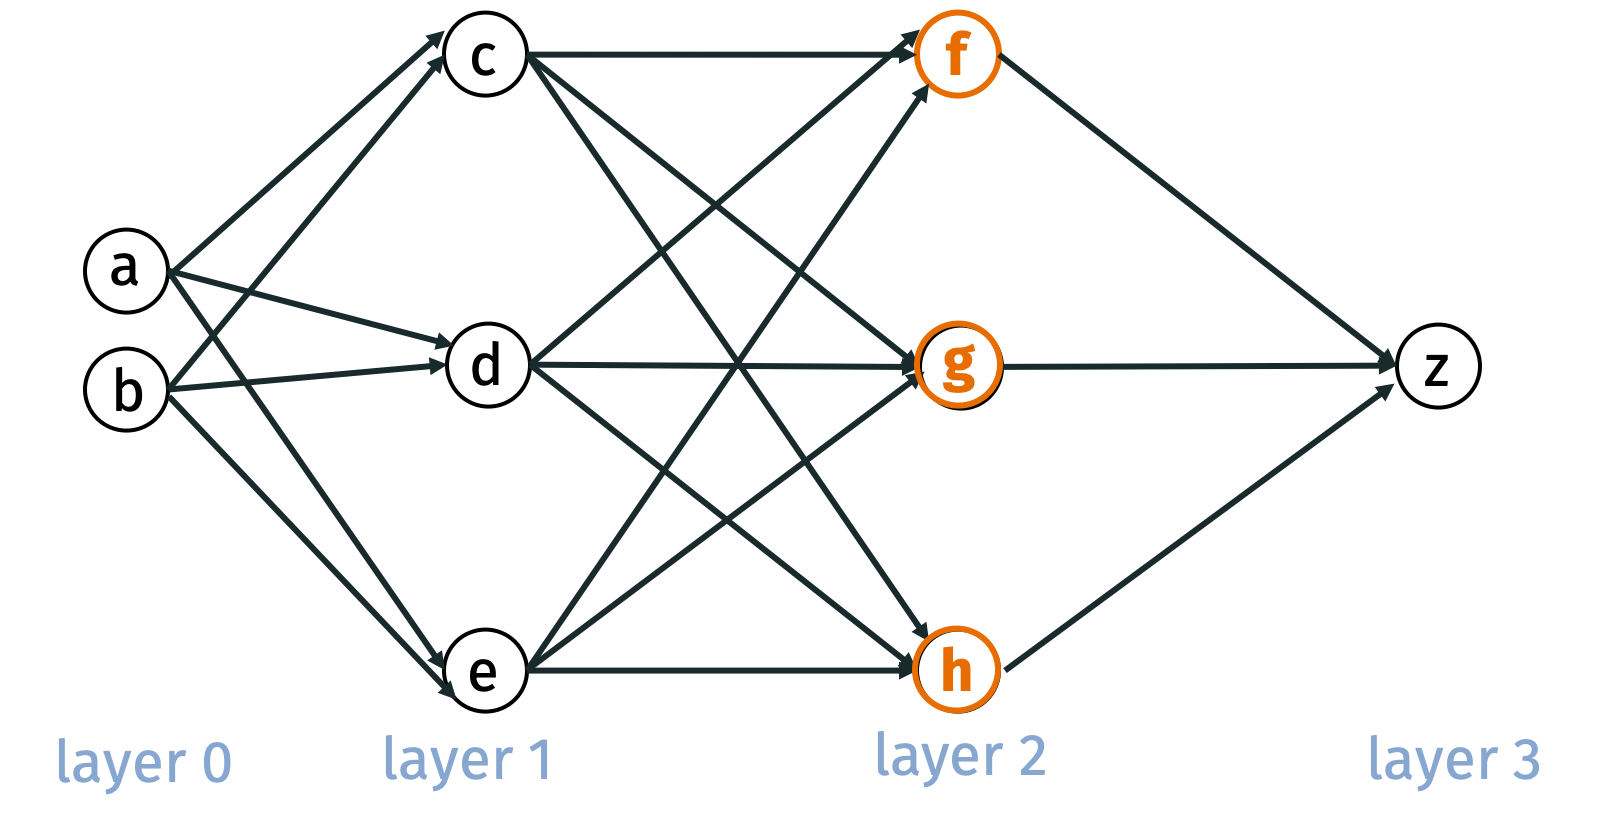
\includegraphics[width=.5\textwidth]{nodes1.png}
	\begin{align*}
	\alert{\frac{\partial z}{\partial f}} &= \frac{\partial \bar{z}}{\partial f}\cdot \frac{\partial z}{\partial \bar{z}} = W_{f,z}\cdot s'(\bar{z}) \\
		\alert{\frac{\partial z}{\partial g}} &= \frac{\partial \bar{z}}{\partial g}\cdot \frac{\partial z}{\partial \bar{z}} = W_{g,z}\cdot s'(\bar{z}) \\
			\alert{\frac{\partial z}{\partial h}} &= \frac{\partial \bar{z}}{\partial h}\cdot \frac{\partial z}{\partial \bar{z}} = W_{h,z}\cdot s'(\bar{z}) \\
	\end{align*}
	\vspace{-3em}
	
	\begin{center}
		\textbf{\alert{Compute partials with respect to nodes, even though not needed for gradient.}}
	\end{center}
	\end{frame}

	\begin{frame}[t]
	\frametitle{backprop example}
	\small
	\textbf{Step 2:} Backward pass.
	
	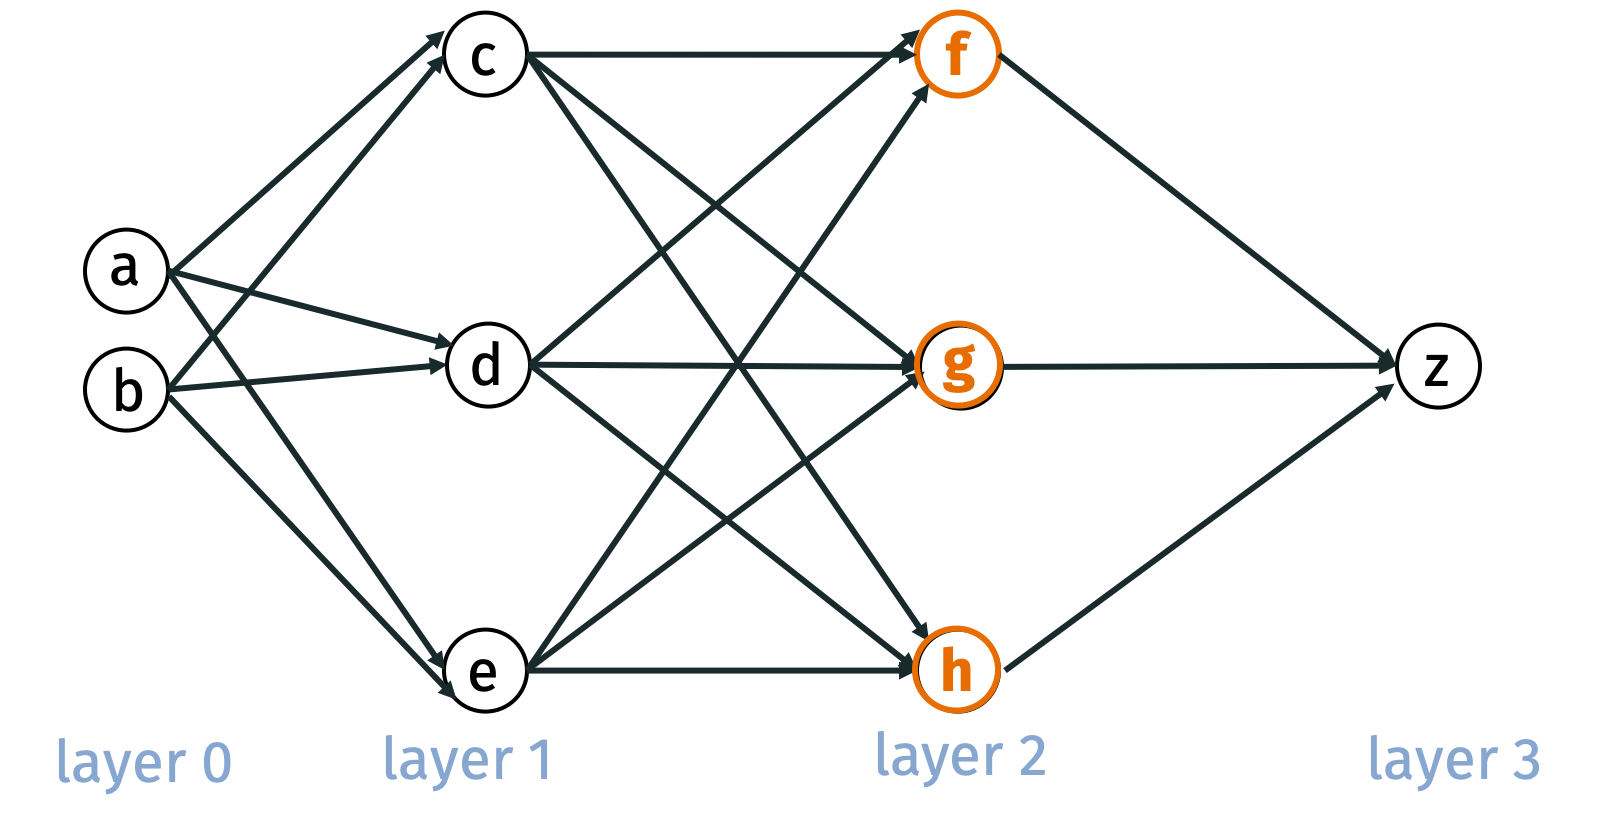
\includegraphics[width=.5\textwidth]{nodes1.png}
	\begin{align*}
	\alert{\frac{\partial z}{\partial \bar{f}}} &= \frac{\partial z}{\partial {f}} \cdot \frac{\partial f}{\partial {\bar{f}}} = \frac{\partial z}{\partial {f}}\cdot s'(\bar{f}) \\
		\alert{\frac{\partial z}{\partial \bar{g}}} &= \frac{\partial z}{\partial {g}} \cdot \frac{\partial g}{\partial {\bar{g}}} = \frac{\partial z}{\partial {g}}\cdot s'(\bar{g}) \\
			\alert{\frac{\partial z}{\partial \bar{h}}} &= \frac{\partial z}{\partial {h}} \cdot \frac{\partial h}{\partial {\bar{h}}} = \frac{\partial z}{\partial {h}}\cdot s'(\bar{h}) \\
	\end{align*}
	\vspace{-3em}
	
	\begin{center}
		\textbf{\alert{And for nodes pre-nonlinearity}}
	\end{center}
\end{frame}
	
	\begin{frame}[t]
	\frametitle{backprop example}
	\small
	\textbf{Step 2:} Backward pass. Next layer.
	
	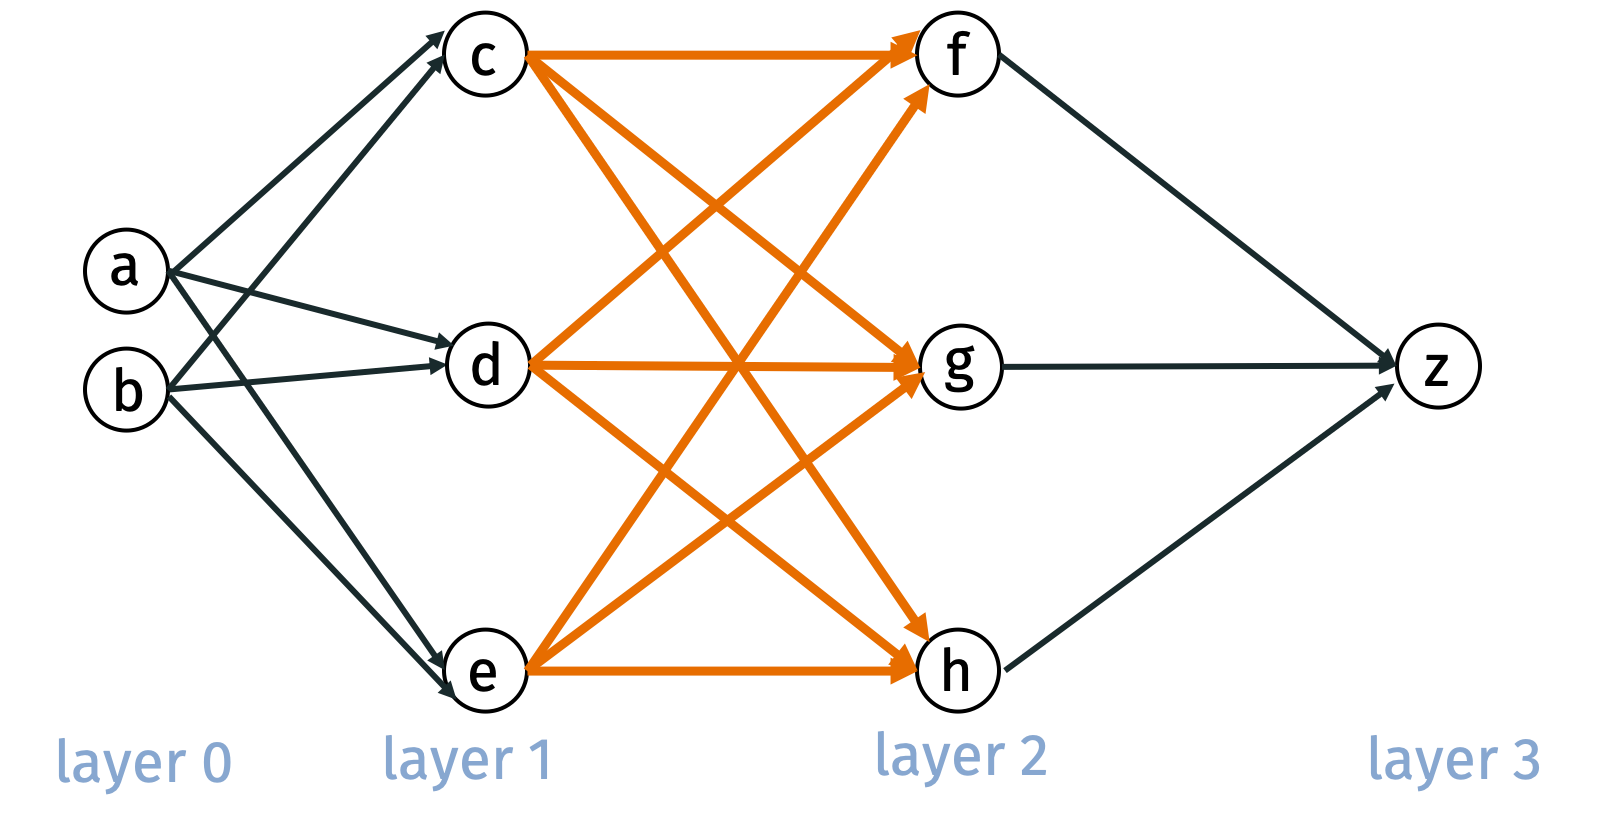
\includegraphics[width=.5\textwidth]{layer2.png}
	\begin{align*}
	\alert{\frac{\partial z}{\partial b_{f}}} &= \frac{\partial z}{\partial \bar{f}}\cdot \frac{\partial \bar{f}}{\partial b_f} = \frac{\partial z}{\partial \bar{f}} \cdot 1\\
	\alert{\frac{\partial z}{\partial W_{c,f}}} &= \frac{\partial z}{\partial \bar{f}}\cdot \frac{\partial \bar{f}}{\partial W_{c,f}} = \frac{\partial z}{\partial \bar{f}}\cdot c\\
		\alert{\frac{\partial z}{\partial W_{d,f}}} &= \frac{\partial z}{\partial \bar{f}}\cdot \frac{\partial \bar{f}}{\partial W_{d,f}} = \frac{\partial z}{\partial \bar{f}}\cdot d\\
			\alert{\frac{\partial z}{\partial W_{e,f}}} &= \frac{\partial z}{\partial \bar{f}}\cdot \frac{\partial \bar{f}}{\partial W_{e,f}} = \frac{\partial z}{\partial \bar{f}}\cdot e\\
		&\vdots
	\end{align*}
\end{frame}

	\begin{frame}[t]
	\frametitle{backprop example}
	\small
	\textbf{Step 2:} Backward pass. Next set of nodes.
	
	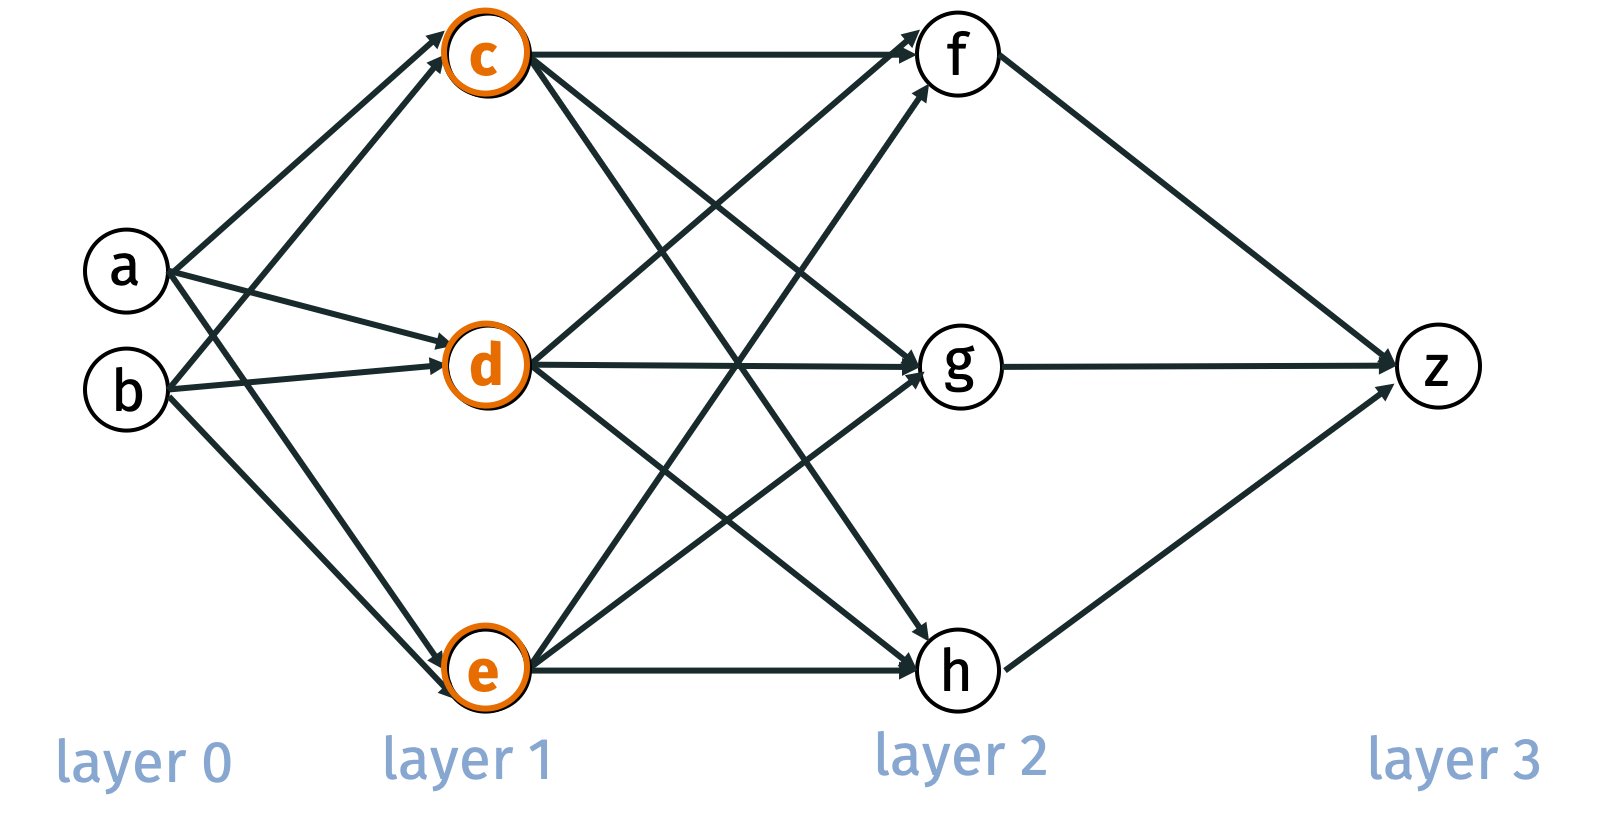
\includegraphics[width=.5\textwidth]{nodes2.png}
	\begin{align*}
	\alert{\frac{\partial z}{\partial c}} &= \frac{\partial z}{\partial \bar{f}}\cdot \frac{\partial \bar{f}}{\partial c} + \frac{\partial z}{\partial \bar{g}}\cdot \frac{\partial \bar{g}}{\partial c} + \frac{\partial z}{\partial \bar{h}}\cdot \frac{\partial \bar{h}}{\partial c}\\
	\alert{\frac{\partial z}{\partial d}} &= \frac{\partial z}{\partial \bar{f}}\cdot \frac{\partial \bar{f}}{\partial d} + \frac{\partial z}{\partial \bar{g}}\cdot \frac{\partial \bar{g}}{\partial d} + \frac{\partial z}{\partial \bar{h}}\cdot \frac{\partial \bar{h}}{\partial d}\\
	\alert{\frac{\partial z}{\partial e}} &= \frac{\partial z}{\partial \bar{f}}\cdot \frac{\partial \bar{f}}{\partial e} + \frac{\partial z}{\partial \bar{g}}\cdot \frac{\partial \bar{g}}{\partial e} + \frac{\partial z}{\partial \bar{h}}\cdot \frac{\partial \bar{h}}{\partial e}
	\end{align*}
	\vspace{-1em}
	
	\begin{center}
		\textbf{Multivariate chain rule:} Need to sum up impact on gradient from all variables effected in the next layer.
	\end{center}
\end{frame}

	\begin{frame}
	\frametitle{backprop linear algebra}
	\small
	\textbf{Linear algebraic view}. 
	
	Let $\bv{v}_i$ be a vector containing the value of all nodes $j$ in layer $i$. 
	\begin{align*}
	\bv{v}_3 &= \begin{bmatrix}z\end{bmatrix} & \bv{v}_2 &= \begin{bmatrix}f\\ g\\h\end{bmatrix} & \bv{v}_1 &= \begin{bmatrix} c\\d\\ e\end{bmatrix} 
	\end{align*}
	Let $\bar{\bv{v}}_i$ be a vector containing $\bar{j}$ for all nodes $j$ in layer $i$. 
	\begin{align*}
\bar{\bv{v}}_3 &= \begin{bmatrix}\bar{z}\end{bmatrix} & \bar{\bv{v}}_2 &= \begin{bmatrix}\bar{f}\\ \bar{g}\\\bar{h}\end{bmatrix} & \bar{\bv{v}}_1 &= \begin{bmatrix} \bar{c}\\\bar{d}\\ \bar{e}\end{bmatrix} 
	\end{align*}
	
	\textbf{Note:} $\bv{v}_i = s(\bar{\bv{v}}_i)$ where $s$ is applied entrywise. 
\end{frame}
	
	\begin{frame}
		\frametitle{backprop linear algebra}
		\small
		\textbf{Linear algebraic view}. 
		
		Let $\bs{\delta}_i$ be a vector containing $\partial z /\partial j$ for all nodes $j$ in layer $i$. 
		\begin{align*}
		\bs{\delta}_3 &= \begin{bmatrix}1\end{bmatrix} & \bs{\delta}_2 &= \begin{bmatrix}\partial z /\partial f\\\partial z /\partial g\\\partial z /\partial h\end{bmatrix} & \bs{\delta}_1 &= \begin{bmatrix}\partial z /\partial c\\\partial z /\partial d\\\partial z /\partial e\end{bmatrix} 
		\end{align*}
		Let $\bs{\bar{\delta}}_i$ be a vector containing $\partial z /\partial \bar{j}$ for all nodes $j$ in layer $i$. 
		\begin{align*}
		\bs{\bar{\delta}}_3 &= \begin{bmatrix}\partial z /\partial \bar{z}\end{bmatrix} & \bs{\bar{\delta}}_2 &= \begin{bmatrix}\partial z /\partial \bar{f}\\\partial z /\partial \bar{g}\\\partial z /\partial \bar{h}\end{bmatrix} & \bs{\bar{\delta}}_1 &= \begin{bmatrix}\partial z /\partial \bar{c}\\\partial z /\partial \bar{d}\\ \partial z /\partial \bar{e}\end{bmatrix} 
		\end{align*}
		
		\textbf{Note:} ${\bs{\bar{\delta}}}_i = s'(\bs{\bar{v}}_i) \times \bs{{\delta}}_i$ where $s'$ is the derivative of $s$ and this function, as well as the $\times$ are applied entrywise. 
	\end{frame}
	
	\begin{frame}
		\frametitle{backprop linear algebra}
		\small
		
		Let $\bv{W}_i$ be a matrix containing all the weights for edges between layer $i$ and layer $i+1$. 
		
		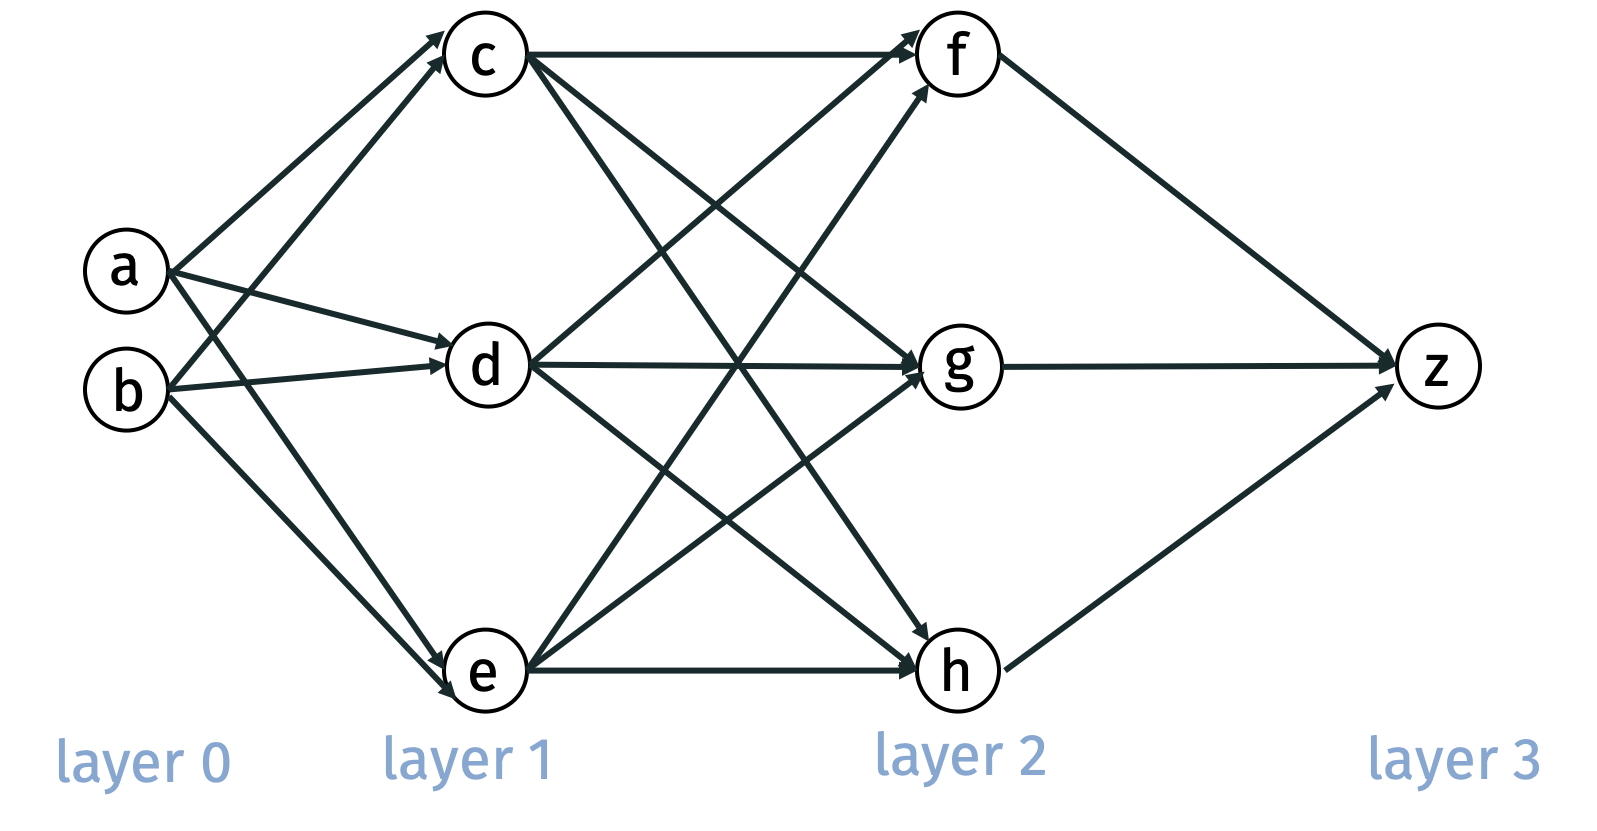
\includegraphics[width=.5\textwidth]{no_select.png}
		\begin{align*}
		\bv{W}_2 &= \begin{bmatrix}W_{f,z}&W_{g,z}& W_{h,z}\end{bmatrix} & \bv{W}_1 &= \begin{bmatrix}W_{c,f}&W_{d,f}& W_{e,f}\\
		W_{c,g}&W_{d,g}& W_{e,g}\\
		W_{c,h}&W_{d,h}& W_{e,h}
		\end{bmatrix}
		& \bv{W}_0 &= \begin{bmatrix}W_{a,c}&W_{b,c}\\
		W_{a,d}&W_{b,d}\\
		W_{a,e}&W_{b,e}
		\end{bmatrix}
		\end{align*}
	\end{frame}
	
	\begin{frame}
		\frametitle{backprop linear algebra}
		\small
		
		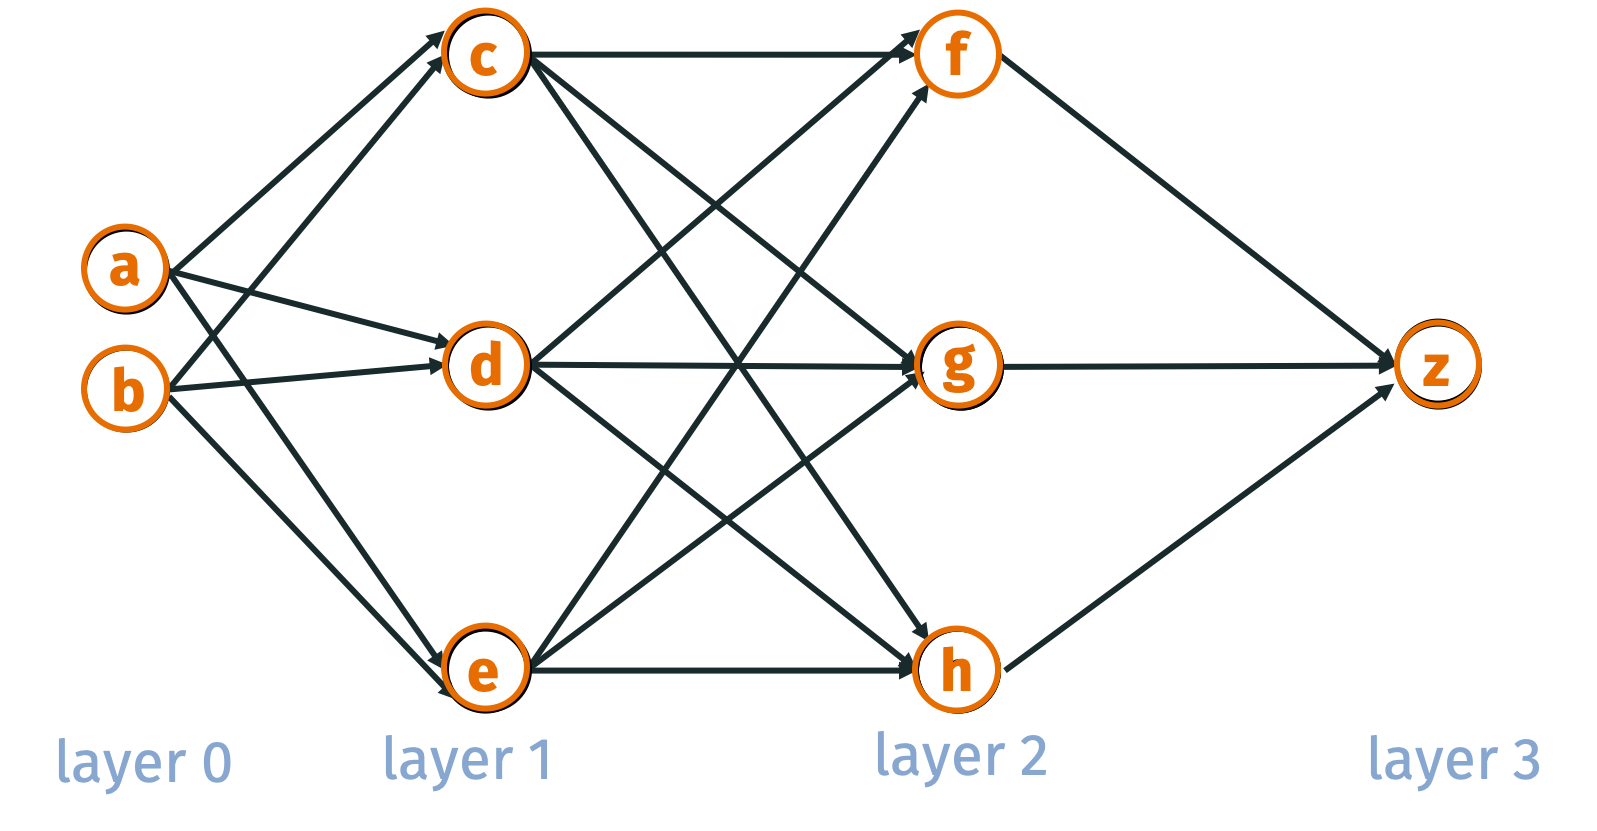
\includegraphics[width=.5\textwidth]{all_nodes.png}
		
		\textbf{Claim 1:} Node derivative computation is matrix multiplication.
		\begin{align*}
		\vec{\delta}_i = \bv{W}_i^T \bar{\delta}_{i+1}
		\end{align*}
	\end{frame}
	
	\begin{frame}
		\frametitle{backprop linear algebra}
		\small
		
		Let $\bs{\Delta}_i$ be a matrix contain the derivatives for all weights for edges between layer $i$ and layer $i+1$. 
		
		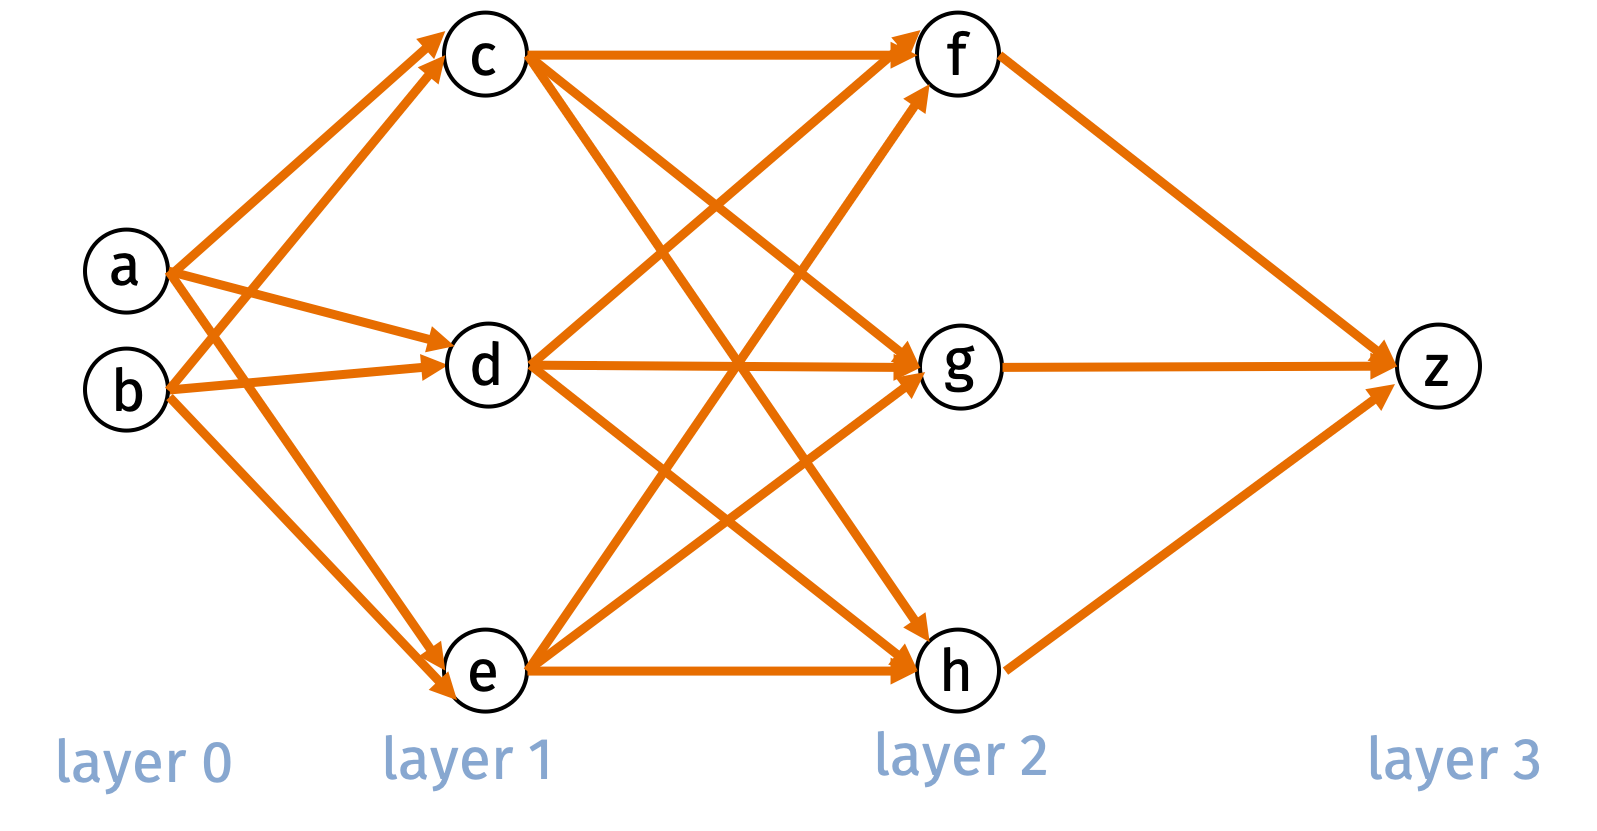
\includegraphics[width=.5\textwidth]{all_edges.png}
		\begin{align*}
		\bs{\Delta}_2 &= \begin{bmatrix}\partial z/\partial W_{f,z}&\partial z/\partial W_{g,z}& \partial z/\partial W_{h,z}\end{bmatrix} \\
		\bs{\Delta}_1 &= \begin{bmatrix}\partial z/\partial W_{c,f}&\partial z/\partial W_{d,f}& \partial z/\partial W_{e,f}\\
		\partial z/\partial W_{c,g}&\partial z/\partial W_{d,g}& \partial z/\partial W_{e,g}\\
		\partial z/\partial W_{c,h}&\partial z/\partial W_{d,h}& \partial z/\partial W_{e,h}
		\end{bmatrix}\\
		\bs{\Delta}_0 &= \ldots
		\end{align*}
	\end{frame}
	
	\begin{frame}
		\frametitle{backprop linear algebra}
		\small
		
		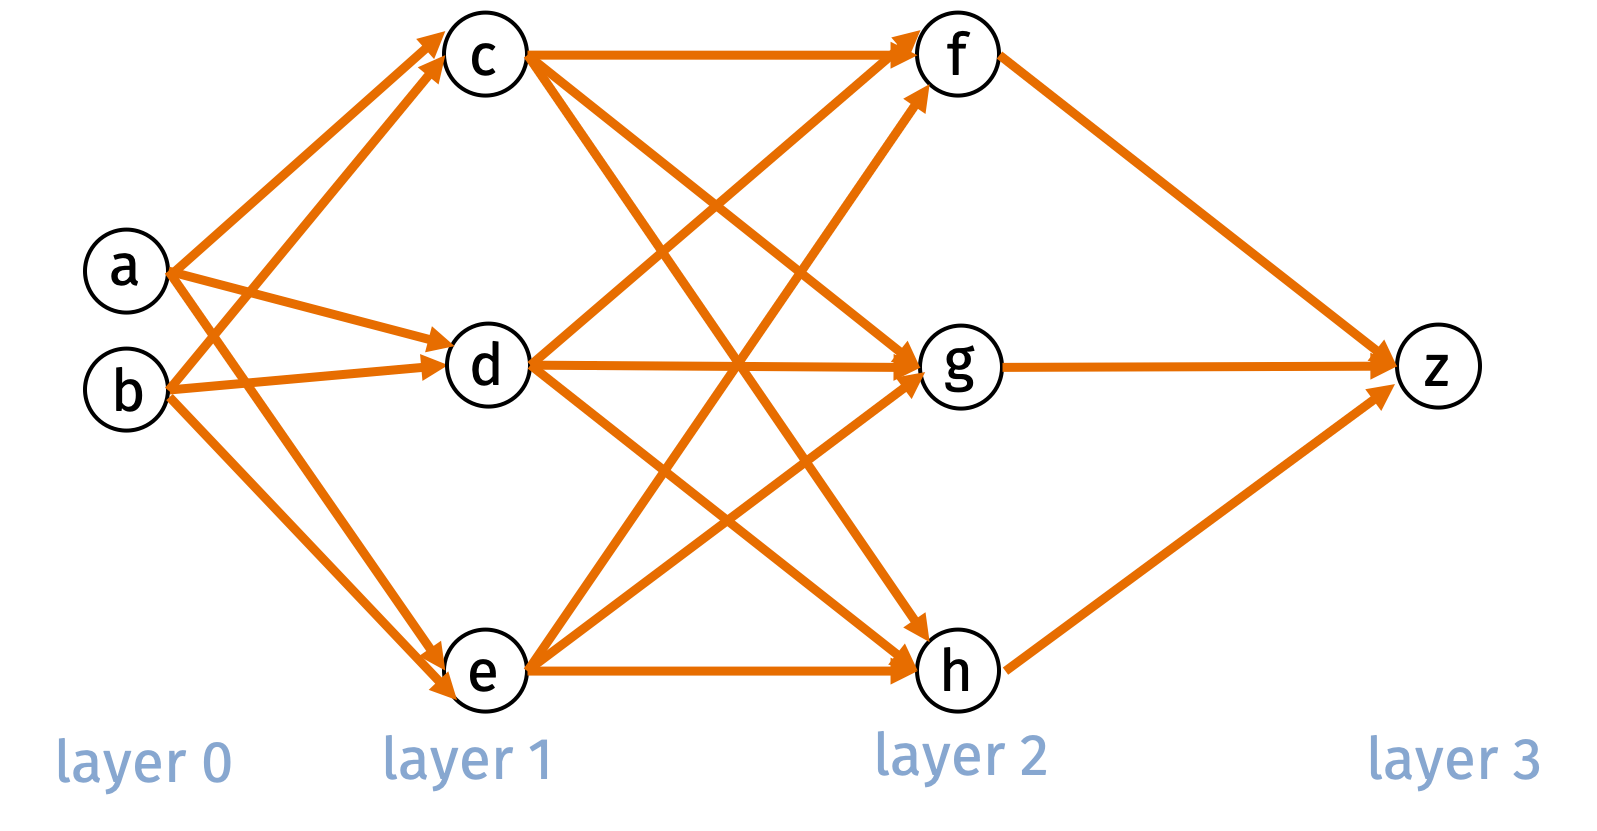
\includegraphics[width=.5\textwidth]{all_edges.png}
		
		\textbf{Claim 2:} Weight derivative computation is an outer-product.
		\begin{align*}
		\bs{\Delta}_i = \bv{v}_i\bar{\delta}_{i+1}^T.
		\end{align*}
	\end{frame}
	
	\begin{frame}
		\frametitle{backprop}
		\textbf{Takeaways:}
		\begin{itemize}
			\item Backpropagation can be used to compute derivatives for all weights and biases for any feedforward neural network.
			\item Final computation boils down to linear algebra operations (matrix multiplication and vector operations) which can be performed quickly on a GPU.
		\end{itemize}
	\end{frame}

	\begin{frame}
	\frametitle{backprop}
	Backpropagation allows us to compute $\nabla L\left(y_i,f(\vec{\theta}, \vec{x}_i)\right)$ for a \emph{single training example} $(\vec{x}_i, y_i)$. Computing entire gradient requires computing:
	\begin{align*}
	\nabla \mathcal{L}(\vec{\theta}) = \sum_{i=1}^n \nabla L\left(y_i,f(\vec{\theta},\vec{x}_i)\right)
	\end{align*}
	\begin{center}
		\textbf{Computing the entire sum would be very expensive.}
		$O\left((\text{time for backprop})\cdot n\right)$ time.
	\end{center}
\end{frame}
	
	\begin{frame}
		\frametitle{training neural networks}
		\textbf{Second tool:} Stochastic Gradient Descent (SGD).
		\begin{itemize}
			\item Powerful {randomized} variant of gradient descent used to train neural networks. \item Or any other model where \emph{computing gradients is expensive}.
		\end{itemize}
		\vspace{2em}
		\textbf{Recall gradient descent update:}
		\begin{itemize}
			\item For $t = 1, \ldots, T$:
			\begin{itemize}
				\item $\vec{\theta}_{t+1} = \vec{\theta}_{t} - \eta \nabla \mathcal{L}(\vec{\theta}_t)$
			\end{itemize}
		\end{itemize}
		where $\eta$ is a learning rate parameter. 
	\end{frame}
	
	\begin{frame}
		\frametitle{stochastic gradient descent}
		Let $L_j(\vec{\theta})$ denote $L\left(y_j,f(\vec{\theta},\vec{x}_j)\right)$.
		
		\textbf{Claim:} If $j \in 1, \ldots, n$ is chosen uniformly at random. Then:
		\begin{align*}
		n\cdot\E\left[\nabla L_j(\vec{\theta}) \right] = \nabla \mathcal{L}(\vec{\theta}).
		\end{align*}
		\vspace{5em}
		
		$\nabla L_j(\vec{\theta})$ is called a \textbf{\alert{stochastic gradient}}.
	\end{frame}
	
	\begin{frame}
		\frametitle{stochastic gradient descent}
		\textbf{SGD iteration:}
		\begin{itemize}
			\item Initialize $\vec{\theta}_0$ (typically randomly).
			\item For $t = 1, \ldots, T$:
			\begin{itemize}
				\item Choose $j$ uniformly at random.
				\item Compute stochastic gradient $\vec{g} = \nabla L_j(\vec{\theta_t})$.
				\begin{itemize}
					\item For neural networks this is done using backprop with training example $(\vec{x}_j, y_j)$. 
				\end{itemize}
				\item Update $\vec{\theta}_{t+1} = \vec{\theta}_{t} - \eta \vec{g}$
			\end{itemize}
		\end{itemize}
		\begin{center}
			\textbf{\alert{Move in direction of steepest descent \emph{in expectation.}}}
		\end{center}
	\end{frame}
	
	\begin{frame}
		\frametitle{stochastic gradient descent}
		\textbf{Gradient descent:} Fewer iterations to converge, higher cost per iteration.
		
		\textbf{Stochastic Gradient descent:} More iterations to converge, lower cost per iteration.
		
		\begin{center}
			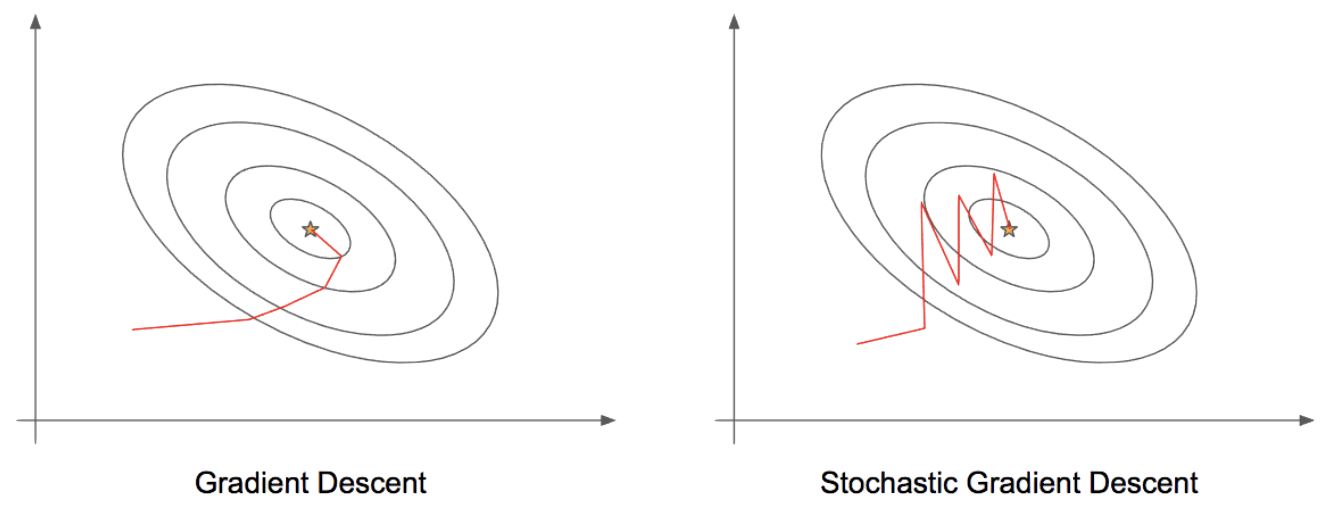
\includegraphics[width=\textwidth]{sgd_path_tame.png}
		\end{center}
	\end{frame}
	
	\begin{frame}
		\frametitle{stochastic gradient descent}
		\textbf{Gradient descent:} Fewer iterations to converge, higher cost per iteration.
		
		\textbf{Stochastic Gradient descent:} More iterations to converge, lower cost per iteration.
		
		\begin{center}
			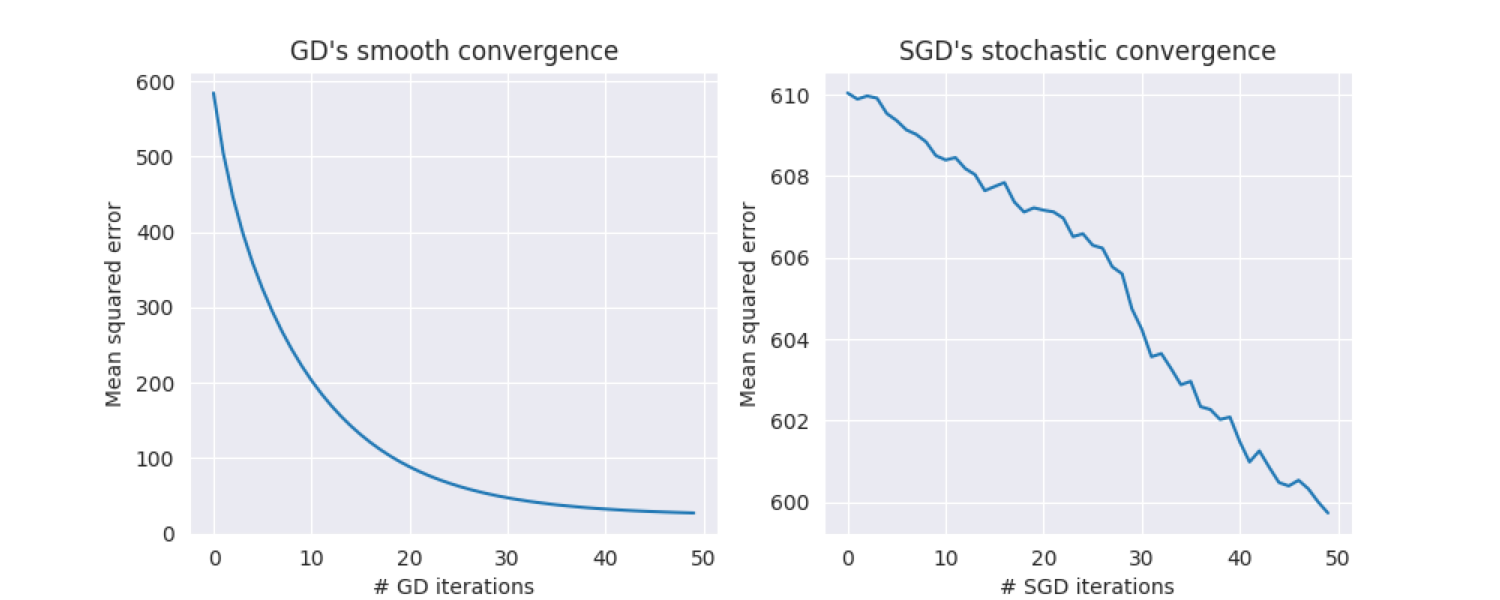
\includegraphics[width=.9\textwidth]{gd_convergence.png}
		\end{center}
	\end{frame}

\begin{frame}
	\frametitle{convergence}
	\small
		 Like standard gradient descent, stochastic gradient descent is only \emph{guaranteed} to converge to the minimizer of a \emph{convex loss function.} 
		\begin{definition}[Convex]
			A function $L$ is convex iff for any $\vec{\beta_1}, \vec{\beta_2},\lambda \in [0,1]$:
			\begin{align*}
			(1-\lambda)\cdot L(\vec{\beta_1}) + \lambda \cdot L(\vec{\beta_2}) \geq L\left((1-\lambda)\cdot\vec{\beta_1}+ \lambda \cdot\vec{\beta_2}\right)
			\end{align*}
			\vspace{-1em}
		\end{definition}
		\vspace{-2em}
		\begin{center}
			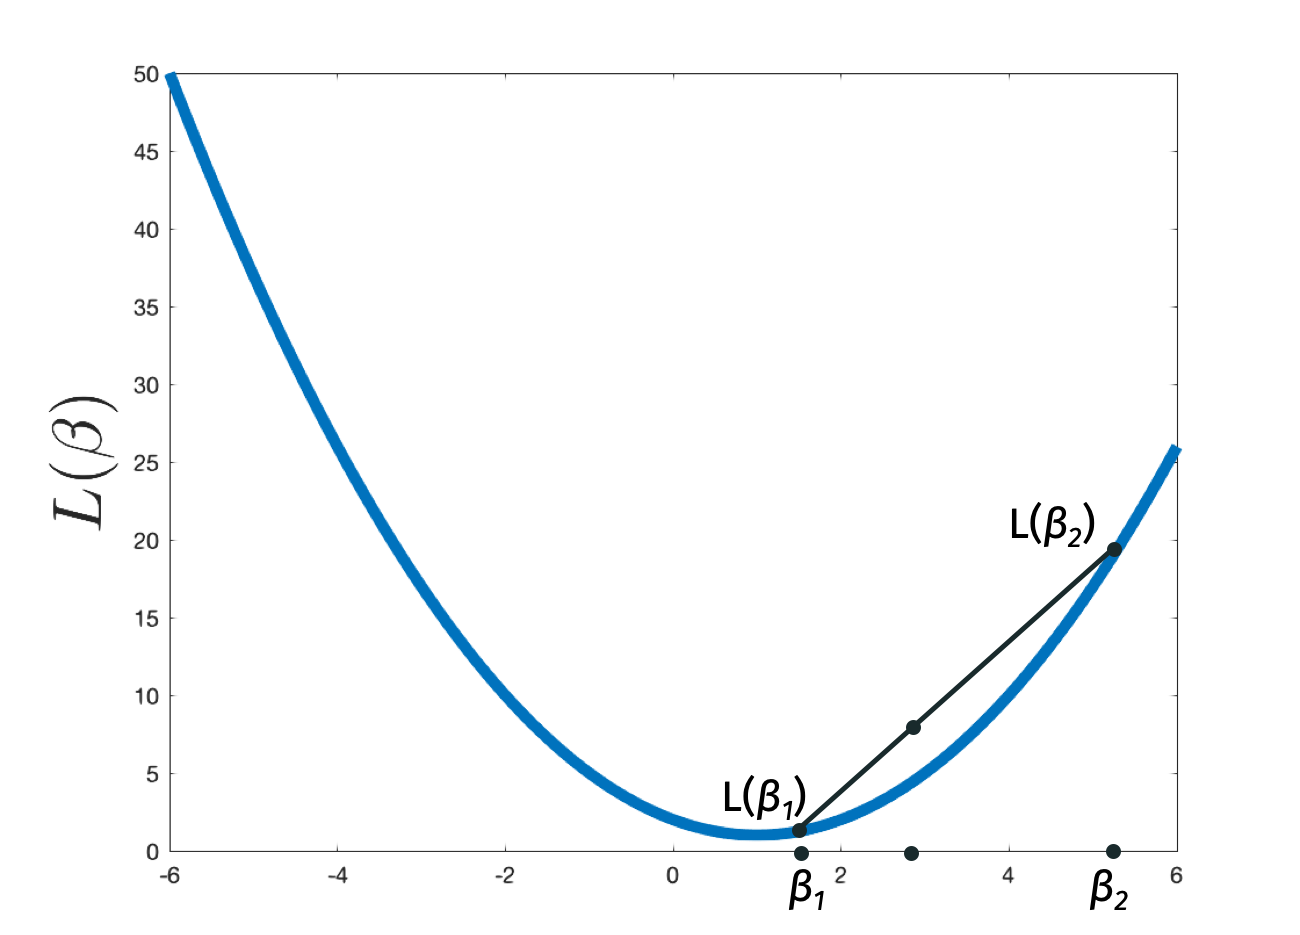
\includegraphics[width=.5\textwidth]{convex.png}
		\end{center}
\end{frame}

\begin{frame}[t]
	\frametitle{convergence of gradient descent}
	\begin{center}
		Without convexity, we can only expect to converge to a local minimum.
		
		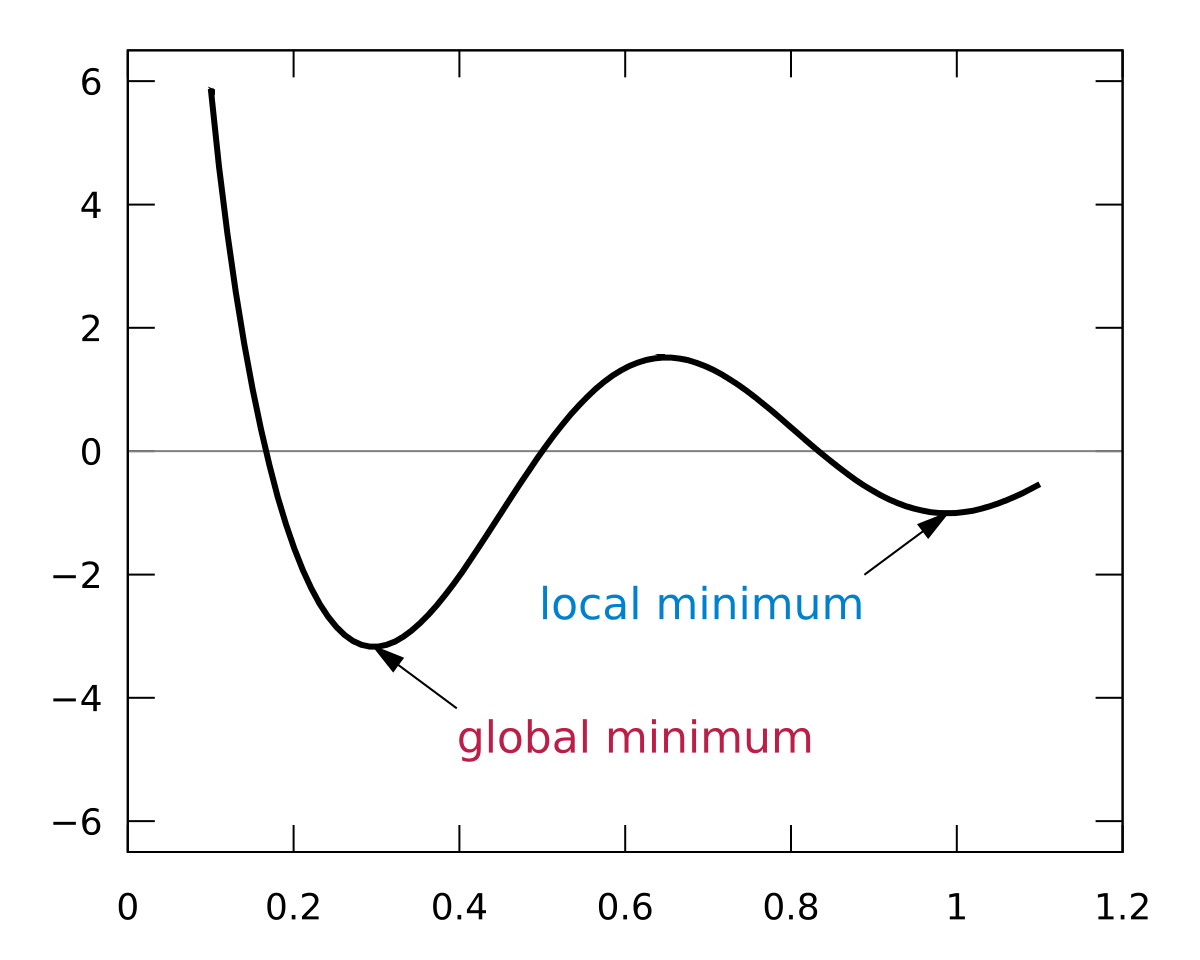
\includegraphics[width=.7\textwidth]{local_min.png}
	\end{center}
\end{frame}


\begin{frame}
	\frametitle{convergence}
	Least squares regression, logistic regression, SVMs, even all of these with kernels lead to convex losses.
	\begin{center}
		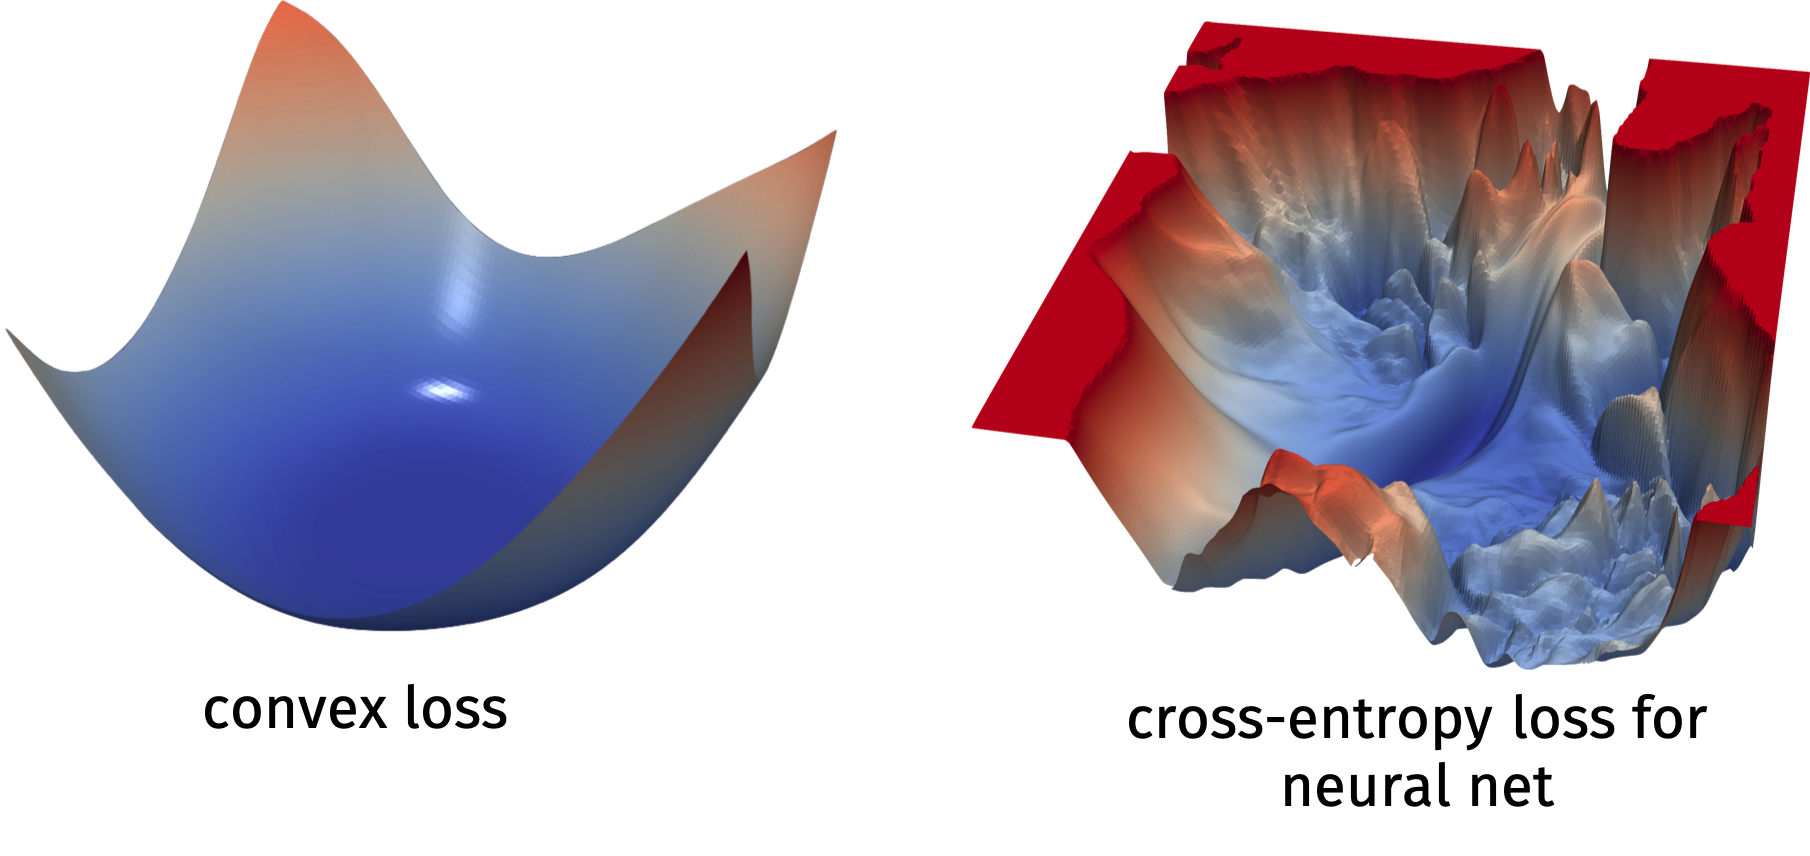
\includegraphics[width=.8\textwidth]{nonconvex.png}
	\end{center}

Neural networks very much do not...
	
\end{frame}

\begin{frame}
	\frametitle{convergence}
	\small
	But SGD still performs remarkably well in practice. Understanding this phenomenon is a major open research question in machine learning and soptimization. Current hypotheses include:
	\begin{itemize}
		\item Initialization seems important (random uniform vs. random Gaussian vs. Xavier initialization vs. He initialization vs. etc.)
		\item Randomization helps in  escaping local minima.
		\item All local minima are global minima?
		\item SGD finds ``good'' local minima?
	\end{itemize}
	\begin{center}
	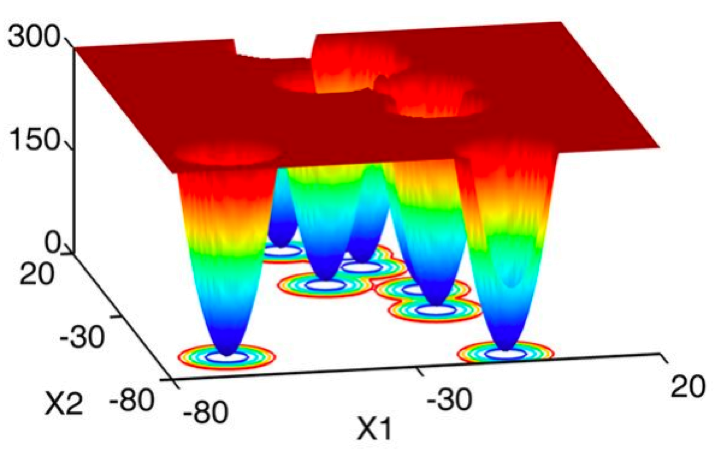
\includegraphics[width=.4\textwidth]{localminglobal.png}
\end{center}
	
\end{frame}
	
	\begin{frame}
		\frametitle{stochastic gradient descent in practice}
		\emph{Practical Modification 1: \textbf{Shuffled Gradient Descent.}}
		
		Instead of choosing $j$ randomly at each iteration, randomly permute (shuffle) data and set $j= 1, \ldots, n$. After every $n$ iterations, reshuffle data and repeat.
		
		\textbf{Question:} Why might we want to do this?
		
	\end{frame}

	\begin{frame}
	\frametitle{stochastic gradient descent in practice}
	\emph{Practical Modification 1: \textbf{Shuffled Gradient Descent.}}
	
			Instead of choosing $j$ randomly at each iteration, randomly permute (shuffle) data and set $j= 1, \ldots, n$. After every $n$ iterations, reshuffle data and repeat.
	
	\begin{itemize}
		\item Relatively similar convergence behavior to standard SGD. 
		\item \textbf{Important term:} one \alert{\textbf{epoch}} denotes one pass over all training examples: $j= 1, \ldots, j=n$. 
		\item Convergence rates for training neural networks are often discussed in terms of epochs instead of iterations. 
	\end{itemize}
\end{frame}
	
	\begin{frame}
		\frametitle{stochastic gradient descent in practice}
		\emph{Practical Modification 2: \textbf{Mini-batch Gradient Descent.}}
		
		Observe that for any \emph{batch size} $s$,
		\begin{align*}
		n\cdot\E\left[\frac{1}{s}\sum_{i=1}^s\nabla L_{j_i}(\vec{\theta}) \right] = \nabla \mathcal{L}(\vec{\theta}).
		\end{align*}
		if $j_1, \ldots, j_s$ are chosen independently and uniformly at random from $1, \ldots, n$.
		
		Instead of computing a full stochastic gradient, compute the average gradient of a small random set (a \emph{mini-batch}) of training data examples. 
		
		\textbf{Question:} Why might we want to do this?
		
	\end{frame}
	
	\begin{frame}
		\frametitle{mini-batch gradient descent}
		\begin{center}
			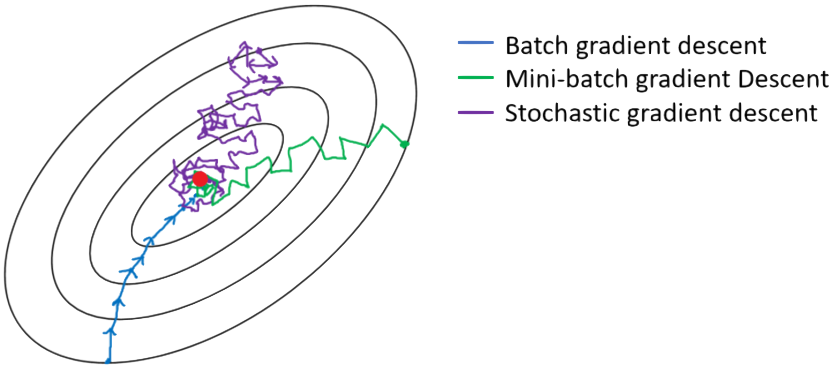
\includegraphics[width=.7\textwidth]{sgd_v_batch.png}
		\end{center}
		\begin{itemize}
			\item For small batch size $s$, mini-batch gradients are nearly as fast to compute as stochastic gradients (due to parallelism).  
			\item Overall faster convergence (fewer iterations needed). 
		\end{itemize}
		
	\end{frame}

	\begin{frame}
	\frametitle{stochastic gradient descent in practice}
	\emph{Practical Mod. 3: \textbf{Per-parameter adaptive learning rate.}}
	
	Let $\vec{g} = \begin{bmatrix}g_1\\\vdots\\g_p\end{bmatrix}$ be a stochastic or batch stochastic gradient. Our typical parameter update looks like:
	\begin{align*}
	\vec{\theta}_{t+1} = \vec{\theta}_{t} - \eta \vec{g}.
	\end{align*}
	We've already seen a simple method for adaptively choosing the learning rate/step size $\eta$. Worked well for convex functions. 
\end{frame}

	\begin{frame}
	\frametitle{stochastic gradient descent in practice}
	\emph{Practical Mod. 3: \textbf{Per-parameter adaptive learning rate.}}
	
	
	In practice, neural networks can often be optimized much faster by using ``adaptive gradient methods'' like \emph{Adagrad}, \emph{Adadelta}, \emph{RMSProp}, and \alert{\emph{ADAM}}. These methods make updates of the form:
	\begin{align*}
	\vec{\theta}_{t+1} = \vec{\theta}_{t} - \begin{bmatrix}\eta_1 \cdot g_1\\\vdots\\\eta_p\cdot g_p\end{bmatrix}
	\end{align*}
	So we have a separate learning rate for each entry in the gradient (e.g. parameter in the model). And each $\eta_1, \ldots, \eta_p$ is chosen \emph{adaptively.}
\end{frame}
	
	\begin{frame}
		\frametitle{neural network demos}
		\textbf{Two demos uploaded on neural networks:}
		\begin{itemize}
			\item \texttt{keras\_demo\_synthetic.ipynb}
			\item \texttt{keras\_demo\_mnist.ipynb}
		\end{itemize}
		\begin{center}
			Please spend some time working through these!
		\end{center}
	\end{frame}

	\begin{frame}
	\frametitle{neural network software}
	\small
	\begin{center}
		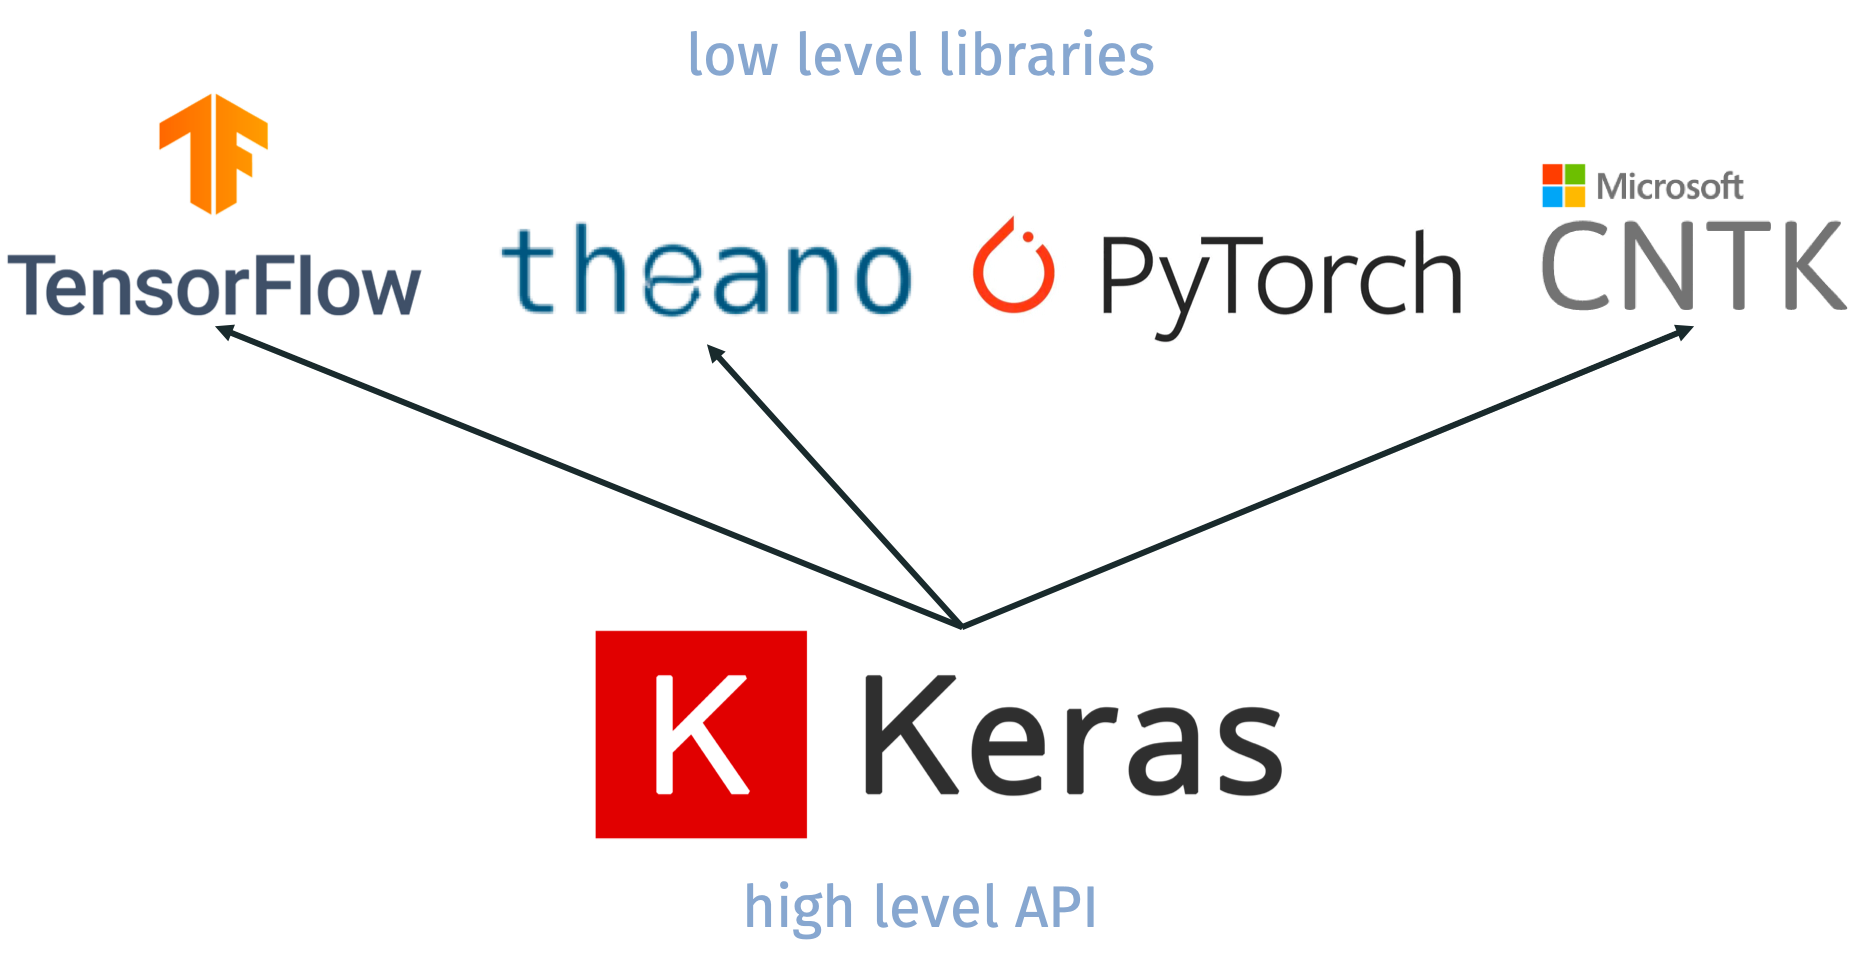
\includegraphics[width=.9\textwidth]{neural_net_zoo.png}
	\end{center}
	\vspace{-1em}

	\textbf{Low-level libraries} have built in optimizers (SGD and improvements) and can automatically perform backpropagation for arbitrary network structures. Also ptimize code for any available GPUs.
	
	\textbf{Keras} has high level functions for defining and training a neural network architecture.
	\end{frame}
	
	\begin{frame}
		\frametitle{neural network software}
		\small
		\textbf{Define model:}
		\begin{center}
			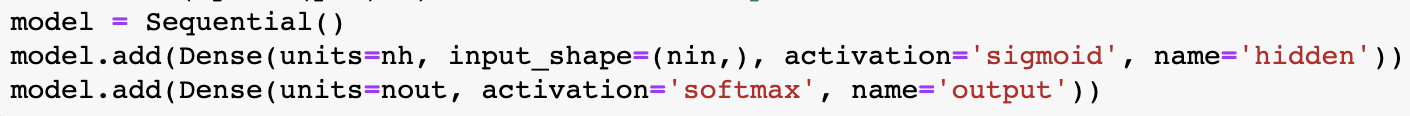
\includegraphics[width=\textwidth]{define_model.png}
		\end{center}
		\vspace{-1em}
		
		\textbf{Compile model:}
		\begin{center}
		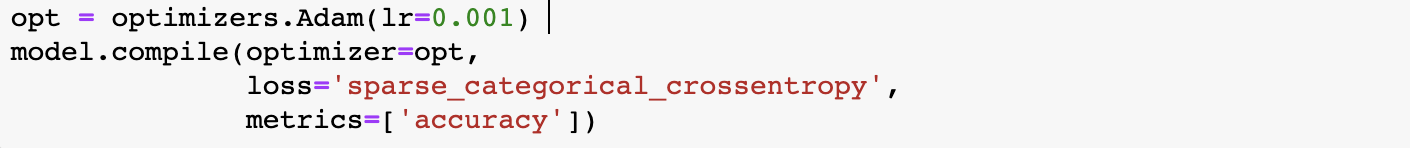
\includegraphics[width=\textwidth]{compile_model.png}
		\end{center}
		\vspace{-1em}
		
		\textbf{Train model:}
		\begin{center}
		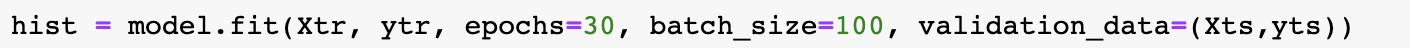
\includegraphics[width=\textwidth]{runmodel.png}
		\end{center}
		\vspace{-1em}
	\end{frame}

	\begin{frame}
	\frametitle{multiclass classification}
	The MNIST lab performs \emph{multiclass classification.} Typically approach to multiclass problems with neural networks is to have one output neuron \emph{per class}:
	\begin{center}
		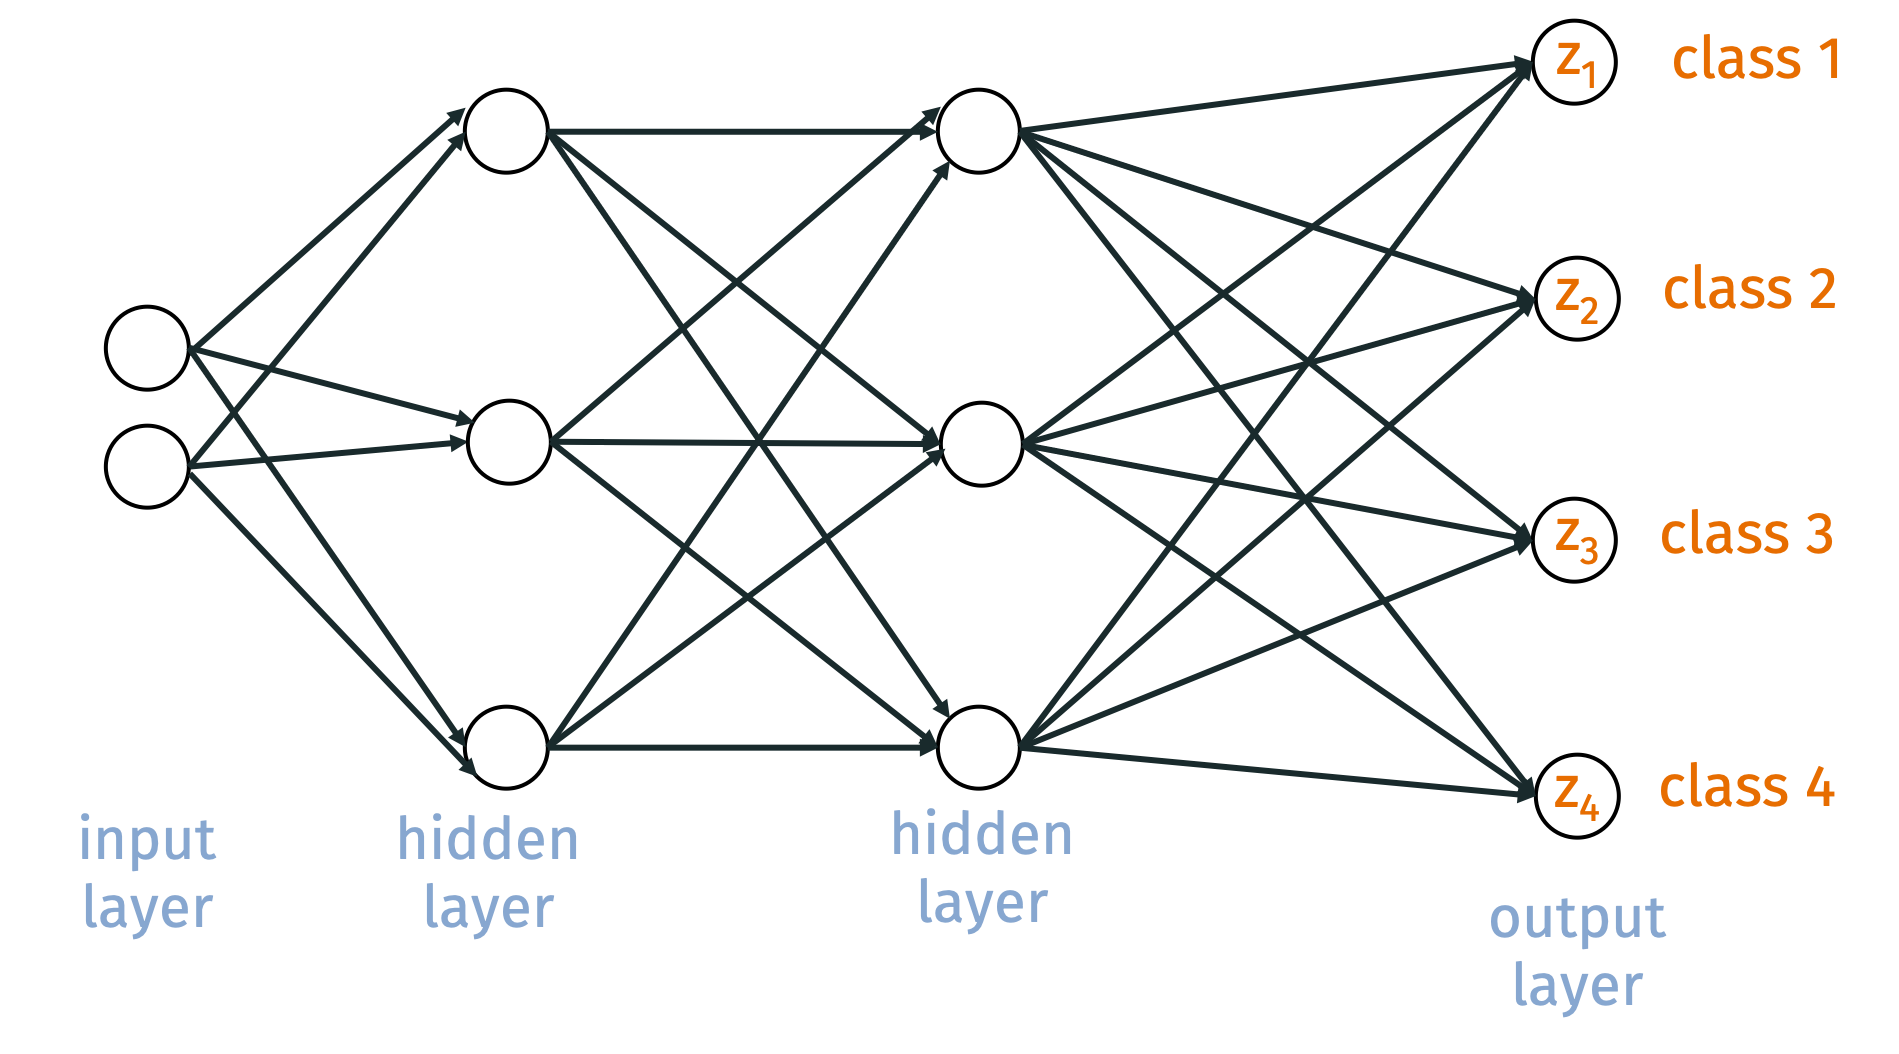
\includegraphics[width=.8\textwidth]{multiclass_network.png}
	\end{center}
	
	\vspace{-1.5em}
	\textbf{Classification rule:} Place in input $\vec{x}$ in class $i$ if $z_i$ is the neuron with maximum value after running $\vec{x}$ through the network.
	\end{frame}

	\begin{frame}
	\frametitle{multiclass classification}
	\begin{center}
		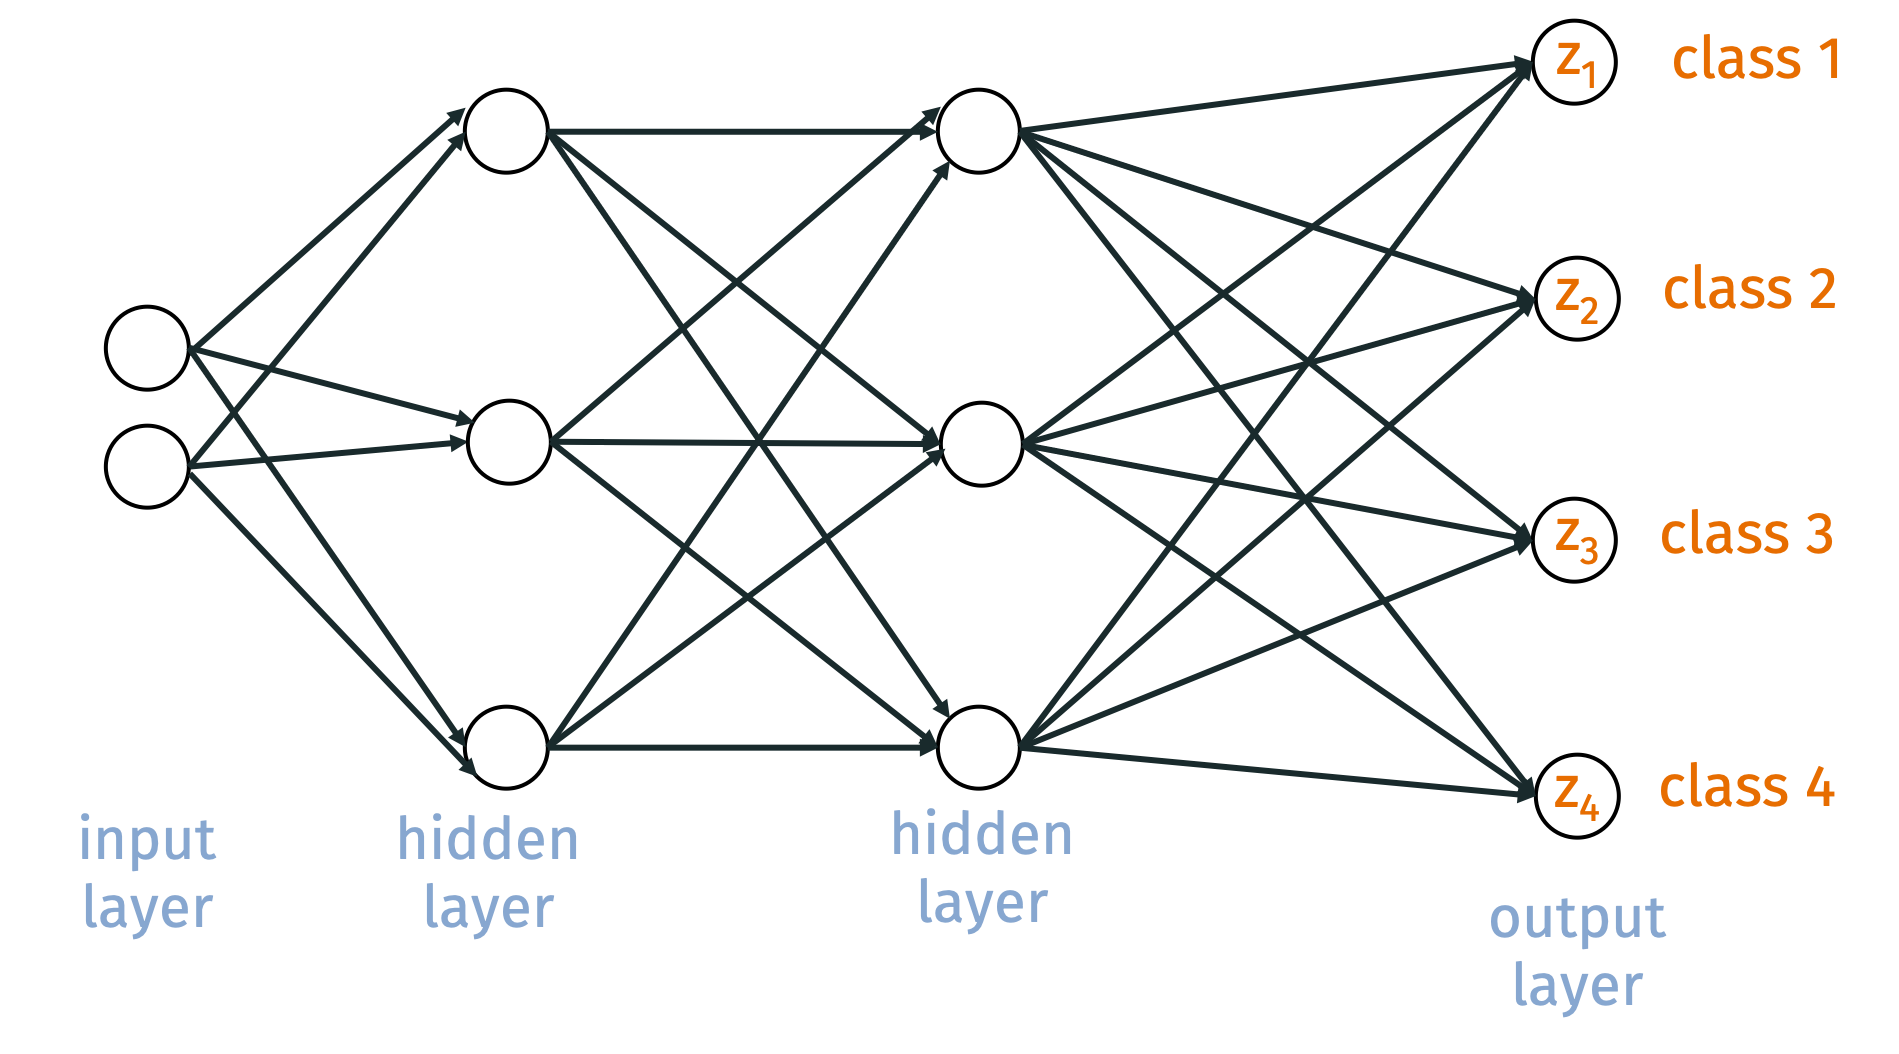
\includegraphics[width=.8\textwidth]{multiclass_network.png}
	\end{center}
Last layer typically uses a ``softmax'' nonlinearity to map all values $\bar{z}_1, \ldots, \bar{z}_q$ to values between $0$ and $1$:
\begin{align*}
z_i = \frac{e^{-\bar{z}_i}}{\sum_{j=1}^q e^{-\bar{z}_j}}.
\end{align*}
	\end{frame}

	\begin{frame}
	\frametitle{multiclass classification}
	Trained using \emph{multiclass cross-entropy loss}. Let $z_1(\vec{x},\theta), \ldots, z_q(\vec{x},\theta)$ be the outputs obtain when running the network on input $\vec{x}$ with parameters (weights and baises) $\vec{\theta}$. 
	\begin{align*}
	L(y, \vec{x}, \vec{\theta}) = - \sum_{i=1}^q \mathbbm{1}[y = i] \log(z_i(\vec{x},\theta)).
	\end{align*}
	
	Overall loss for training data $(\vec{x}_1, y_1), \ldots, (\vec{x}_n, y_n)$ is:
	\begin{align*}
	\mathcal{L}(\vec{\theta}) = \sum_{i=1}^n L(y_i, \vec{x}_i, \vec{\theta})
	\end{align*}
	\begin{center}
		\alert{\textbf{Used in our demo and very standard for neural network classification.}}
	\end{center}
	\end{frame}

\end{document} 



